\documentclass[10pt]{beamer}
\usepackage[utf8]{inputenc}
\usepackage{amsmath}
\usepackage{amsfonts}
\usepackage{amssymb}
\usepackage{graphicx}
\usepackage{alltt}
\usepackage{pdfpages}
\graphicspath{{../sharedfiles/}}

%\usepackage[size=custom,width=27,height=15,scale=1]{beamerposter}
\author{Anthony Odenthal, KE7OSN Amateur Extra}
\title{Technician and General Class Amateur Radio \& Satellite Stuff}
\AtBeginSection[]
{
\begin{frame}
\frametitle{Table of Contents}
\tableofcontents[currentsection]
\end{frame}
}

%\setcounter{tocdepth}{2}
\usetheme{PaloAlto}
\usecolortheme{beetle}
\usepackage{mdwlist}

\begin{document}

\frame{\titlepage}

%\begin{frame}
%\frametitle{Table of Contents}
%\tableofcontents
%\end{frame}

\part{Introduction}

\begin{frame}
\frametitle{Welcome}
Welcome, over the next several sessions we will cover a substantial amount of information. please ask questions and slow me down.\\
The goals are:
\begin{itemize}
\item To introduce you to Amateur Radio \pause
\item Prepare you to take (and pass) the technician and general exams \pause
\item Introduce you to satellite communications.
\end{itemize}
\end{frame}

\begin{frame}
\frametitle{A little about myeself}
\begin{itemize}
%\item I'm a student at Oregon State University %Going to keep to just radio stuff
\item Passed Tech Sept 2007
\item Passed Gen Oct 2007
\item Joined Benton County ARES April 2012
\item Passed Extra April 2012
\item Became a VE in June 2012
\end{itemize}
\end{frame}

\begin{frame}
\frametitle{What is Amateur Radio?}
Amateur radio are people and activities that are regulated and encouraged, in the US and abroad, that allow licensed individuals to play around with radio waves, electronics, software, techniques, practices, and equipment to do all sorts of really cool stuff. Radio Amateurs are some of the least restricted users of radio spectrum, and with that freedom they have proven time and time again their worth.
The term Amateur refers to someone who does something as a pastime rather than a profession.
\end{frame}

\begin{frame}
\frametitle{Some useful tools}
Some things you may want to look into as useful for studying
\begin{itemize}
\item AA9PW practice exams \url{http://aa9pw.com}
\item ARRL license Manuals \url{http://www.arrl.org/shop/Licensing-Education-and-Training/}
\end{itemize}
\end{frame}

\begin{frame}
\frametitle{About the test}
\begin{itemize}
\item 35 questions \pause
\item Multiple Choice \pause
\item No time limit \pause
\item 396 questions in the tech pool, 457 in the general \pause
\item Need a 75\% to pass
\end{itemize}
\end{frame}

\begin{frame}
\frametitle{Shal we begin?}
Remember if I go too fast or you have questions, let me know.
\end{frame}

\part{FCC Rules, descriptions and definitions for the amateur radio service, operator and station license responsibilities}
%\section{T1A - Amateur Radio services; purpose of the amateur service, amateur-satellite service, operator/primary station license grant, where FCC rules are codified, basis and purpose of FCC rules, meanings of basic terms used in FCC rules}
\section{Who's In Charge}
\begin{frame}
\frametitle{Who's In charge}
International Telecommunications Union (ITU)
\begin{itemize}
\item Worldwide, treaty-based organization that allocates frequencies for specific uses.
\item Primary Users - first "rights" to a frequency
\item Secondary Users - permitted to use a frequency but must not interfere with a primary user
\item World divided into 3 regions, US is in Region 2
\item Creates "bands" - sections of spectrum allocated for amateur radio use.
\end{itemize}
\end{frame}

\begin{frame}
\frametitle{Who's In Charge}
Federal Comunications Commission (FCC)
\begin{itemize}
\item Promulgates  rules for non-federal radio users within ITU spec
\item Divides amateur bands into mode-specific sub-bands
\item Rules for telecommunications are in the Code of Federal Regulations, Chapter 47
\item Rules for amateur radio are in Part 97 of Chapter 47 (47 CFR 97)
\end{itemize}
\end{frame}

\begin{frame}
\frametitle{Who's In Charge}
Frequency Coordinator
\begin{itemize}
\item FCC recognized regional groups that coordinate the use of bands between large number of users \pause
\item Appointed by amateurs for amateurs \pause
\item Intended to help reduce and allow resolution of interference issues \pause
\item Voluntary rules unless there is interference, then the coordinated user "wins"\pause
\item Gentleman's agreement
\end{itemize}
\end{frame}

\begin{frame}
\frametitle{FCC allocations}
\begin{center}
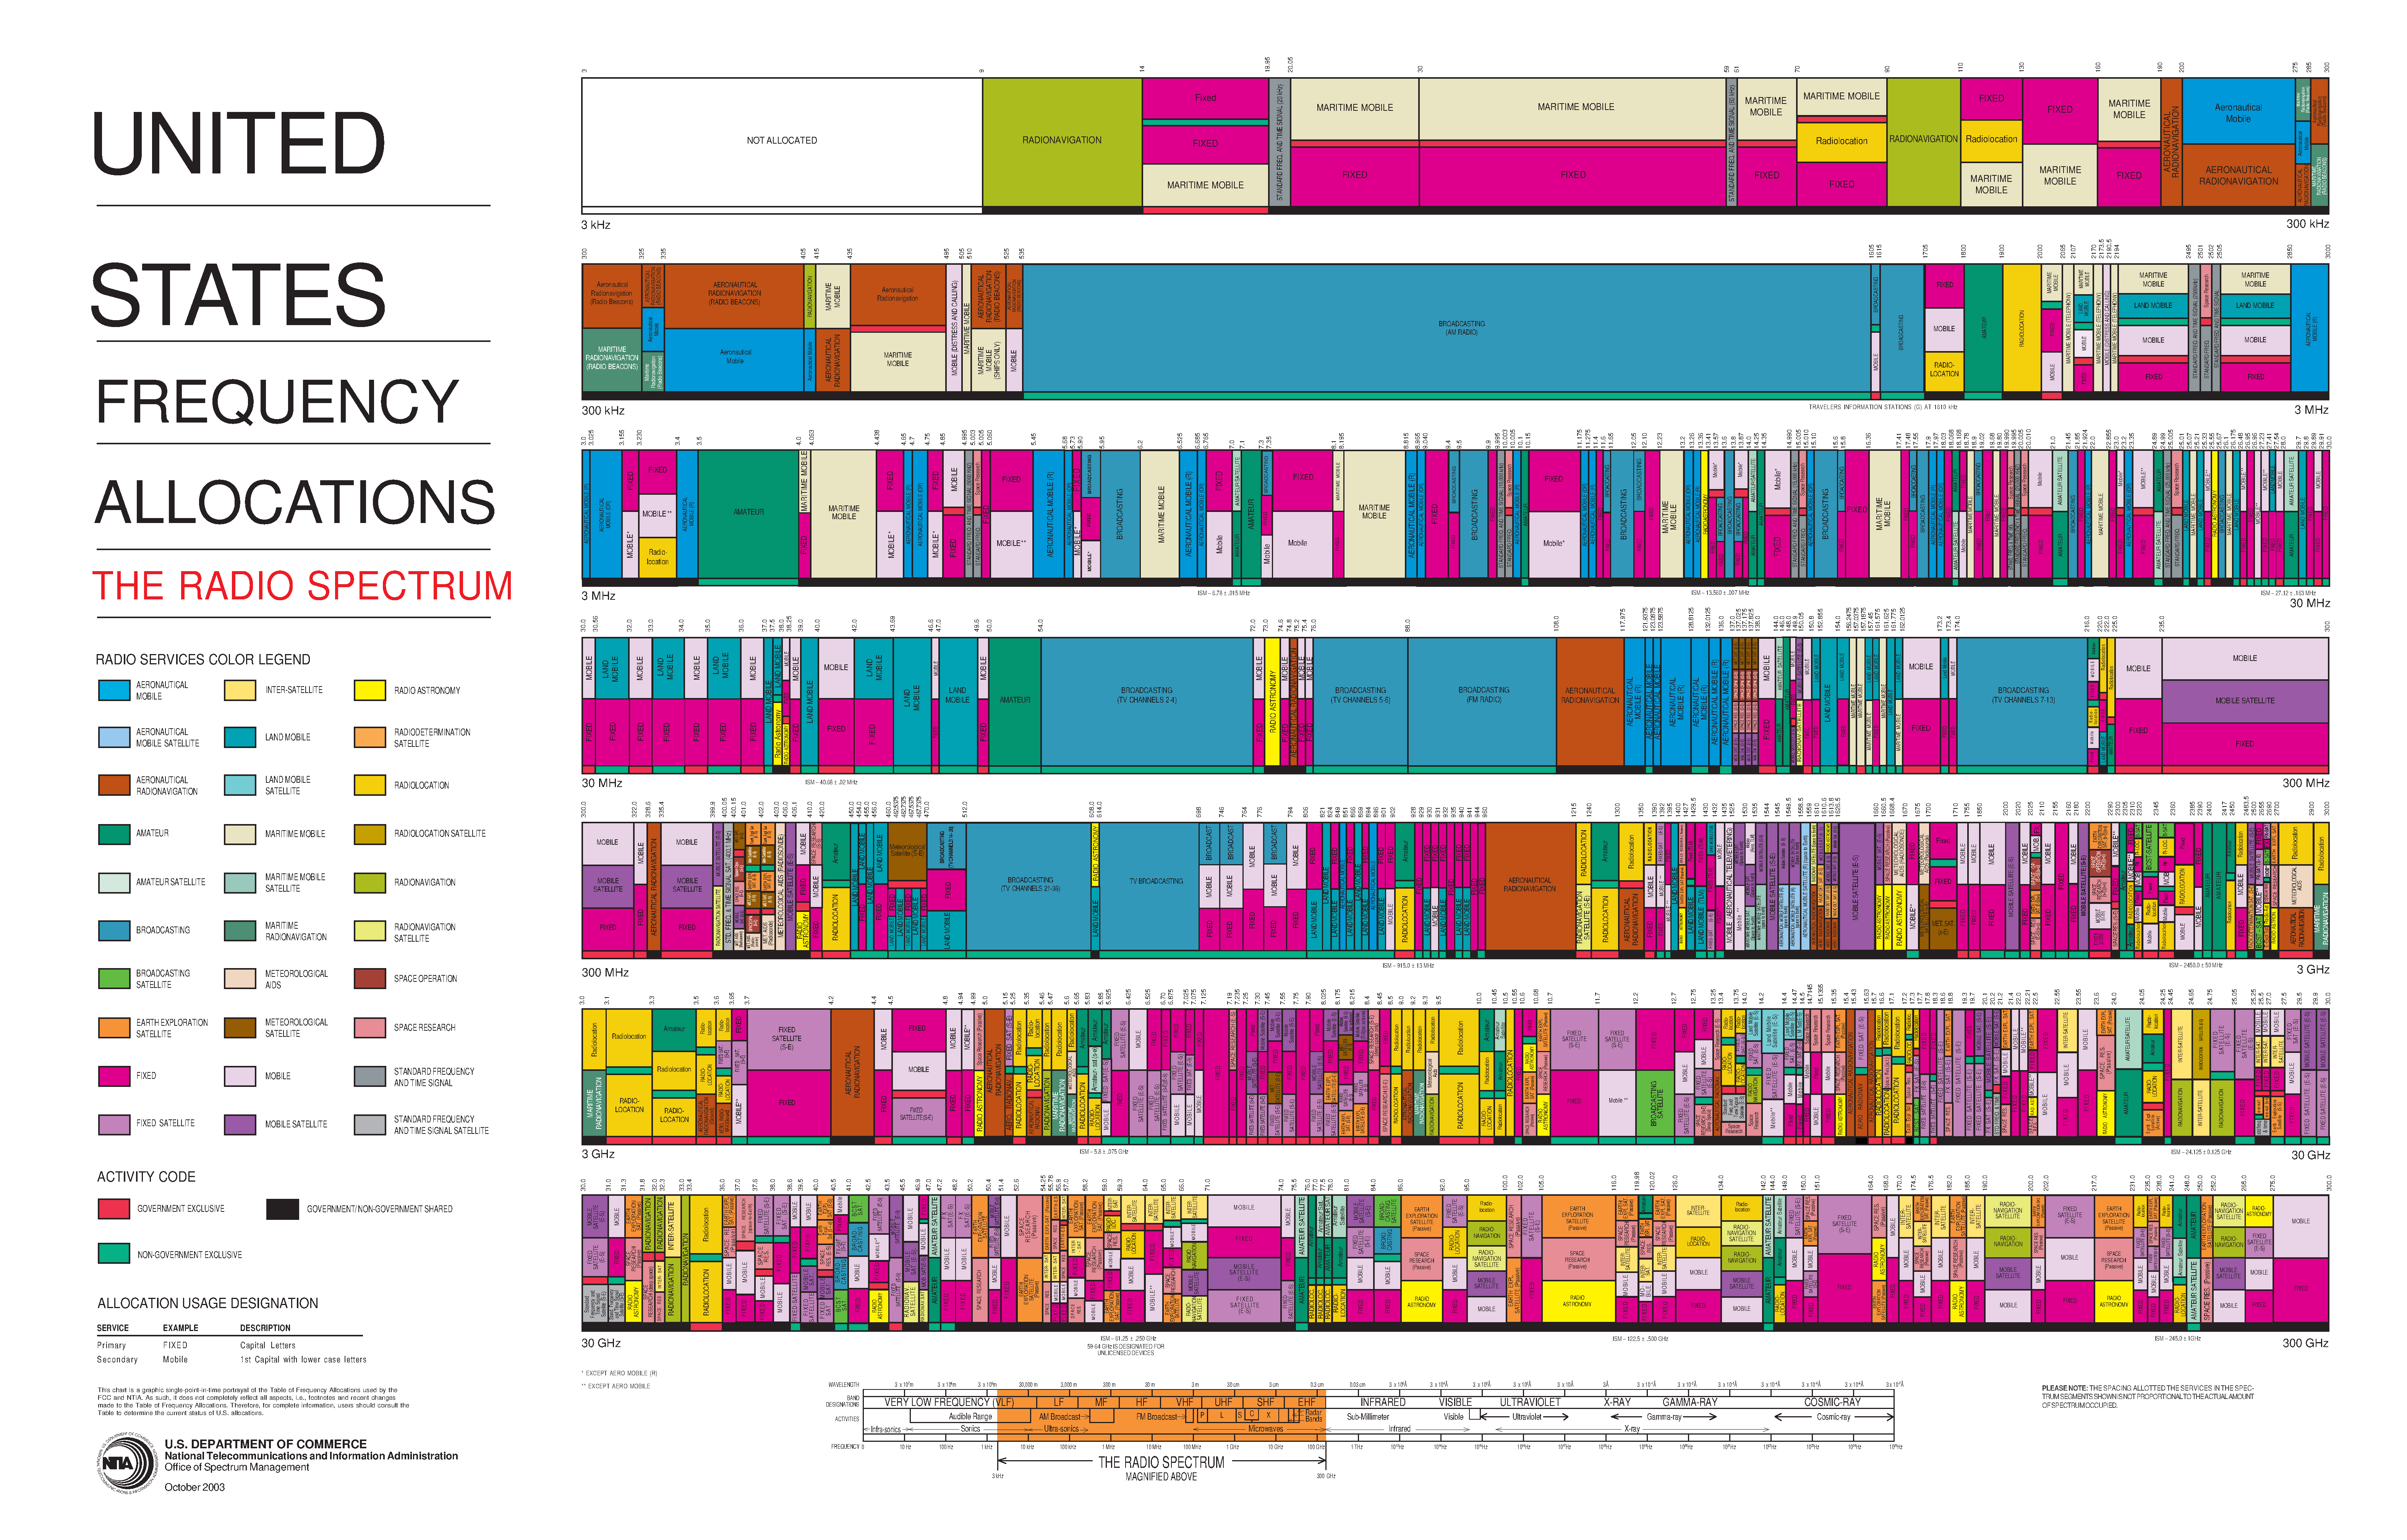
\includegraphics[width=\textwidth]{2003-allochrt.pdf}
\end{center}
\end{frame}

\section{Part 97}

\begin{frame}
\frametitle{47 CRF 97.1 Basic Purpose}
The rules and regulations in this part are designed to provide an amateur radio service having a fundamental purpose as expressed in the following principles:
\begin{enumerate}[A]
\scriptsize\item  Recognition and enhancement of the value of the amateur service to the public as a \emph{voluntary noncommercial communication service}, particularly with respect to providing emergency communications.\pause
\item Continuation and extension of the amateur's proven ability to contribute to the advancement of the radio art.\pause
\item Encouragement and improvement of the amateur service through rules which provide for advancing skills in both the communication and technical phases of the art.\pause
\item  Expansion of the existing reservoir within the amateur radio service of trained operators, technicians, and electronics experts. \pause
\item Continuation and extension of the amateur's unique ability to enhance international goodwill.
\end{enumerate}
\end{frame}

\begin{frame}
\frametitle{Keyphrase}
\begin{alltt}
\ldots\emph{a voluntary noncommercial\\communications service}\ldots
\end{alltt}
This phrase sums up almost every rule and tenant of amateur radio.
\end{frame}

\begin{frame}
\frametitle{A voluntary noncommercial communications service}
Noncommercial means no "pecuniary interest". It is illegal to profit from the use of amateur radio.\\
\hfil \\As with almost any rule there are exceptions"
\begin{itemize}
\item Teachers may use ham radio in the classroom as a teaching aid
\item "Code practice" transmissions
\item Disaster Drills
\end{itemize}
\end{frame}

\begin{frame}
\frametitle{More basic rules}
\begin{itemize}
\item No Music - expect transmission or re-transmission of a signal from a space station
\item No Broadcasting
\item No commercial traffic
\item No profanity
\item No codes or ciphers intended to hid content
\item No international third party traffic unless treaty-approved
\end{itemize}
\end{frame}

\section{licenses}

\begin{frame}
\frametitle{Licenses}
A license is valid for ten years, with a two year grace period. Upgrades don't count as renewals. Basic renewals are free!\\
There are five classes.
\begin{itemize}
\item *Novice
\item Technician
\item General
\item *Advanced
\item Extra
\end{itemize}
\end{frame}

\begin{frame}
\frametitle{Licenses}
There are four kinds of licenses, Individual hams hold both a "Station" and "Operator"
\begin{itemize}
\item Station
\item Operator
\item Club - W7OSU, K7CVO, W1AW
\item Special Event - A7W
\end{itemize}
Clubs can get a "club callsign", and events can get an event callsign.
\end{frame}

\section{Callsigns}

\begin{frame}
\frametitle{Callsigns}
\begin{itemize}
\item US callsigns start with A,K,N, or W
\item The format is one or two letters, a number, and one to three letters.
\item New callsigns are assigned in sequential order - number indicates the region in the US
\item Shorter callsigns are reserved for higher license classes
\item 1X1 for special events only
\end{itemize}
\end{frame}

\begin{frame}
\frametitle{Callsigns}
\begin{itemize}
\item KE7OSN
\item N8GFO \pause -Yep\pause
\item K7HZ \pause -That's an Extra\pause
\item VE6GLW \pause -That's Canadian\pause
\item KLOO \pause -That's a commercial station\pause
\item WSJ509 \pause -Land Mobile, Benton County Sheriff\pause
\item Mission Base \pause -What is known as a "tactical callsign"\pause
\end{itemize}
\end{frame}

%\begin{frame}
%\frametitle{What IS an amateur station?}
%T1A10 (A) [97.3(a)(5)] What is the FCC Part 97 definition of an amateur station?\\ \pause \hfil \\
%A. A station in an Amateur Radio Service consisting of the apparatus necessary for carrying on radio
%communications
%\end{frame}

\begin{frame}
\frametitle{Operator}
Who "operates" an amateur station? \pause \\
The control operator, who is designated by the station licensee, and determines the privileges of operation.\\
e.g.\ if you are at a radio that can operate outside your privileges, you still can only use what you are licensed to.
\end{frame}

\begin{frame}
\frametitle{Your Callsign}
A station must transmit it's callsign at least every ten minutes and at the end of every communication.\\
Special situations have special rules\\
\begin{itemize}
\item Control operator working outside of a station licensee privileges.
\item Special event station control operator
\item Control operator using new privileges prior to FCC database update
\end{itemize}
\end{frame}

\begin{frame}
\frametitle{The Uniform Licensing System}
The ULS is an online database of FCC license information. A new licensee may use their privileges as soon as their information appears in the ULS. When you upgrade you may use your new privileges as soon as you pass the test.
\end{frame}

\begin{frame}
\frametitle{Typical uses of a callsign}
\begin{itemize}[<+->]
\item W7OSU This is KE7OSN
\item Net Control This is KE7OSN
\item This is W7OSU (Go Ahead)
\item CQ CQ CQ this is KE7OSN
\item KE7OSN monitoring
\item This is KF7FGE stroke (/) KE7OSN
\item Hey Bob, you around?
\end{itemize}
\end{frame}

\begin{frame}
\frametitle{Hey bob, you around}
Hey bob you around?\\
Legal? \\ \pause
Yes, as long as you keep to the every ten minutes and the end of every communication. \\ \pause
What if Bob isn't there? \\ \pause
KE7OSN clear
\end{frame}

\begin{frame}
\frametitle{Types of stations}
\begin{itemize}
\item Club – at least four  people, one of which accepts responsibility and is the “trustee”.
\item Space – at least 50km above the surface.
\item Beacon --  transmits a low-level signal for propagation studies
\item Repeater – retransmits  a signal heard on one frequency on another frequency.
\item Auxillary – a secondary receiver that feeds a repeater station.  
\end{itemize}
\end{frame}

\section{frequencies}

\begin{frame}
\frametitle{Band Plan}
\begin{center}
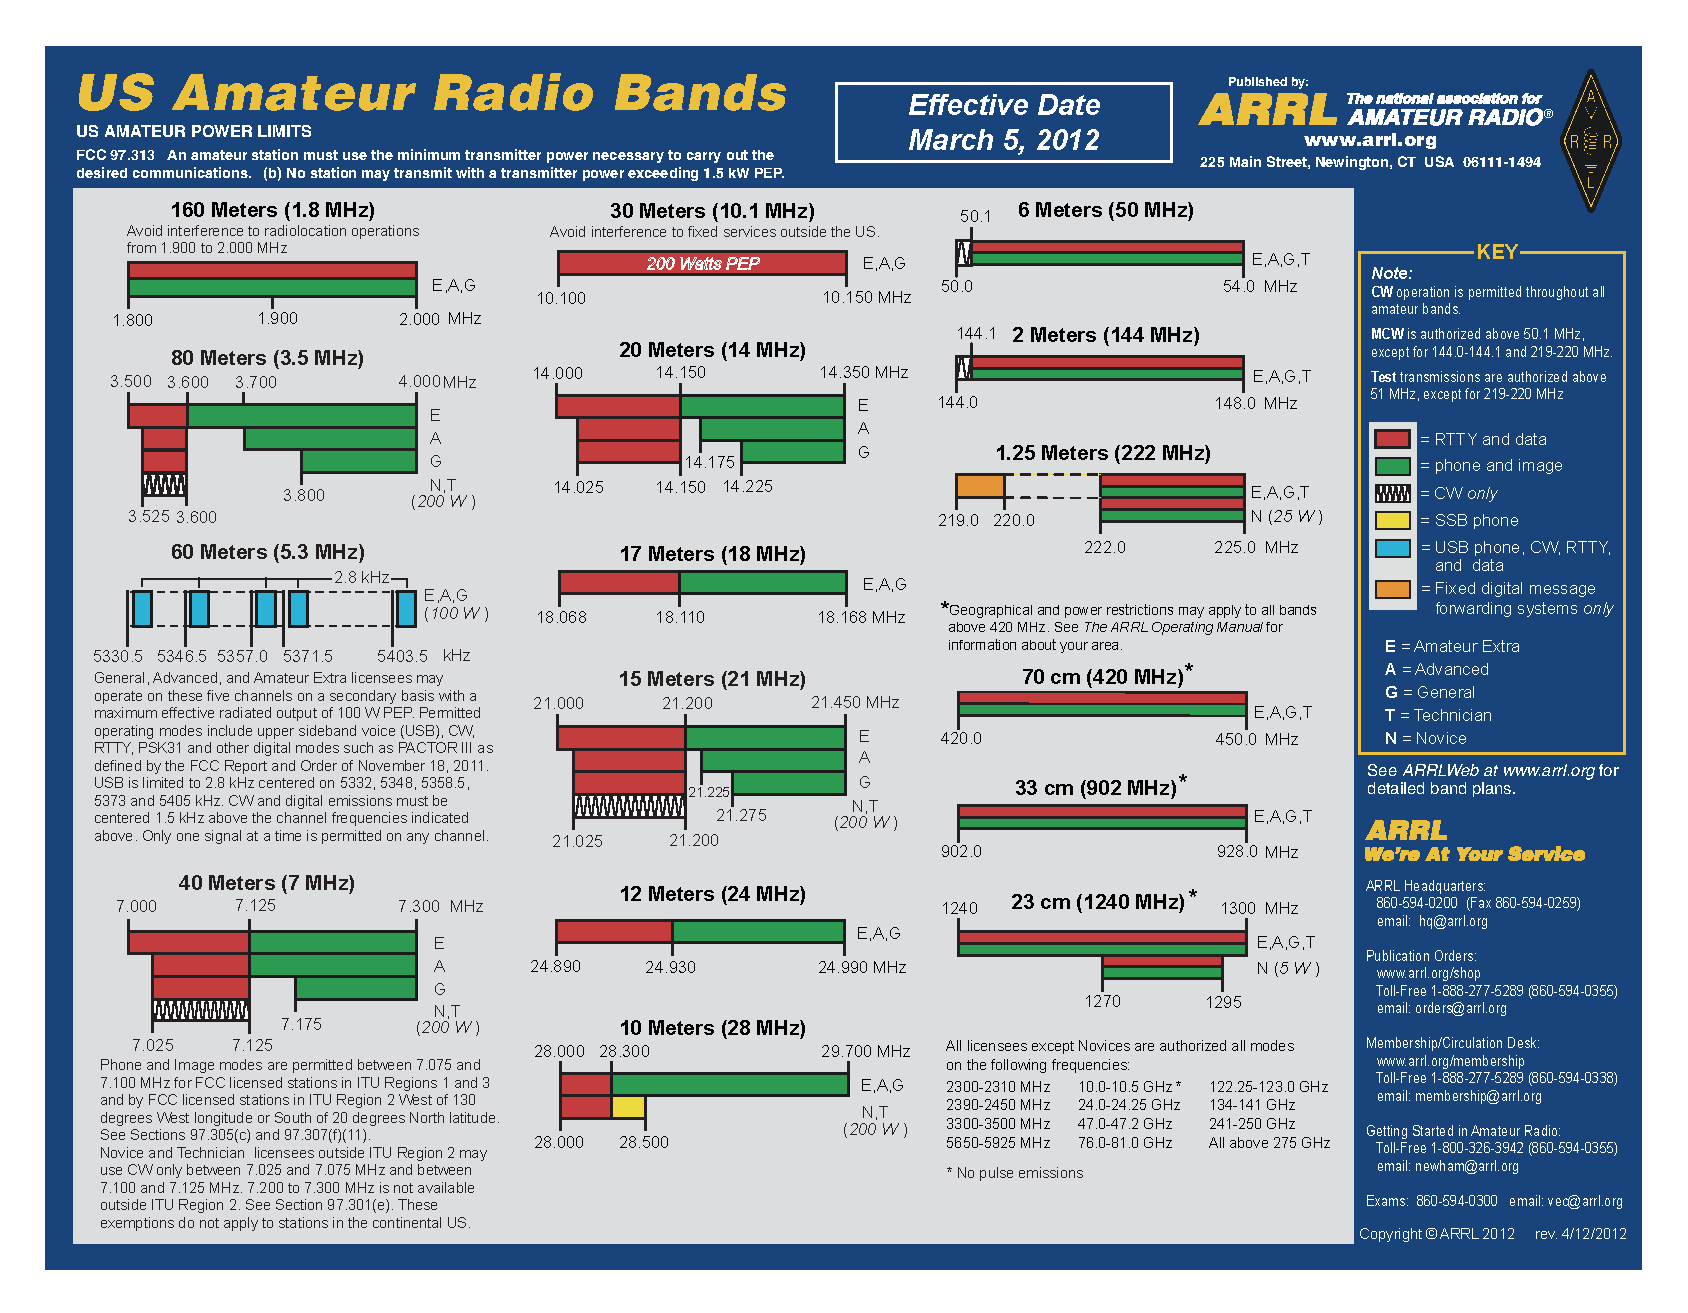
\includegraphics[height=.9\textheight]{hambandscolor.pdf}
\end{center}
\end{frame}

\begin{frame}
\frametitle{ITU Band Names}
\begin{itemize}
\item MF - Medium Frequency 300KHz to 3MHz
\item HF - High Frequency 3MHz to 30 MHz
\item VHF - Very High Frequency 30MHz to 300MHz
\item UHF - Ultra High Frequency 300MHz to 3GHz
\item SHF - Super High Frequency 3GHz to 30GHz
\item EFE - Extremely High Frequency - 30GHz to 300GHz
\item THF - Tremendously High Frequency - 300GHZ to 3THz
\end{itemize}
\end{frame}

\begin{frame}
\frametitle{HF 3-30MHz}
	\begin{itemize}
	\item 80 Meters
		\begin{itemize}
		\item 3.525-3.600MHz: CW Only
		\end{itemize}
	\item 40 Meters
		\begin{itemize}
		\item 7.025-7.125MHz: CW Only
		\end{itemize}
	\item 15 Meters
		\begin{itemize}
		\item 21.025-21.200MHz: CW Only
		\end{itemize}
	\item 10 Meters 
		\begin{itemize}
		\item  28.000-28.300MHz: CW, RTTY/Data 200 watts PEP max 
		\item 28.300-28.500MHz: CW, Phone 200 watts PEP max
		\end{itemize}
	\end{itemize}
\end{frame}

\begin{frame}
\frametitle{VHF 30-300MHz}
	\begin{itemize}
	\item 6 Meters
		\begin{itemize}
		\item 50.0-50.1MHz CW Only
		\item 50.1-54.0MHz All modes
		\end{itemize}
	\item 2 Meters
		\begin{itemize}
		\item  144.0-144.1MHz CW Only
		\item 144.1-148.0MHz All modes
		\end{itemize}
	\item 1.25 Meters
		\begin{itemize}
		\item 222.00-225.00MHz All modes
		\end{itemize}
	\end{itemize}
\end{frame}

\begin{frame}
\frametitle{UHF 300-3000MHz (3GHz)}
\begin{itemize}
\item 70 Centimeters
\begin{itemize}
\item 420.0-450.0MHz All Modes
\end{itemize}
\item 33 Centimeters
\begin{itemize}
\item 902.0-928.0MHz All Modes
\end{itemize}
\item 23 Centimeters
\begin{itemize}
\item 1240-1300MHz All Modes
\end{itemize}
\item 2.4GHz
\begin{itemize}
\item 2.3-2.31GHz
\item 2.39-2.45GHz *
\end{itemize}
\end{itemize}
\end{frame}

\begin{frame}
\frametitle{2.4GHz}
We share the 2390-2450MHz band with: 802.11 networks, cordless phones, video cameras, zigbee, etc.\ \\
We are PRIMARY users. We have first "rights". Secondary users must not cause us interference and must accept interference from our operations.
\end{frame}

\begin{frame}
\frametitle{SHF 3GHz-30GHz and up}
\begin{itemize}
\item 3.3-3.5GHz
\item  5.65-5.925GHz
\item  10.0-10.5GHz
\item  24.0-24.25GHz
\item  47.0-47.2GHz
\item  76.0-81.9GHz
\item  119.98-120.02GHz
\item  142-149GHz
\item  241-250GHz
\item  Everything above 300GHz
\end{itemize}
\end{frame}

\section{T1 Questions}
\subsection{T1A}
\begin{frame}
\frametitle{T1A 6 Questions from T1}
\begin{itemize}[<+->]
\tiny
\item\textbf{T1A01 For whom is the Amateur Radio Service intended?}\hfil \\D. Persons who are interested in radio technique solely with a personal aim and without pecuniary interest
\item\textbf{T1A02 What agency regulates and enforces the rules for the Amateur Radio Service in the United States?} \hfil \\ C. The FCC
\item\textbf{T1A03 Which part of the FCC rules contains the rules and regulations governing the Amateur Radio Service?}\hfil \\ D. Part 97
\item\textbf{T1A04 Which of the following meets the FCC definition of harmful interference?} \hfil \\ C. That which seriously degrades, obstructs, or repeatedly interrupts a radio communication service operating in accordance with the Radio Regulations
\item\textbf{T1A05 What is the FCC Part 97 definition of a space station?} \hfil \\  D. An amateur station located more than 50 km above the Earth’s surface
\item\textbf{T1A06 What is the FCC Part 97 definition of telecommand?}\hfil \\  C. A one-way transmission to initiate, modify or terminate functions of a device at a distance
\item\textbf{T1A07 What is the FCC Part 97 definition of telemetry?}\hfil \\ C. A one-way transmission of measurements at a distance from the measuring instrument
\item\textbf{T1A08 Which of the following entities recommends transmit/receive channels and other parameters for auxiliary and repeater stations?}\hfil \\B. Frequency Coordinator
\item\textbf{T1A09 Who selects a Frequency Coordinator?}\hfil \\ C. Amateur operators in a local or regional area whose stations are eligible to be auxiliary or repeater stations
\item\textbf{T1A10 What is the FCC Part 97 definition of an amateur station?}\hfil \\ A. A station in an Amateur Radio Service consisting of the apparatus necessary for carrying on radio communications
\item\textbf{T1A11 Which of the following stations transmits signals over the air from a remotereceive site to a repeater for retransmission?} \hfil \\C. Auxiliary station
\end{itemize}
\tiny 11 of 396 2.7\%
\end{frame}
\subsection{T1B}
\begin{frame}
\frametitle{T1B 6 Questions from T1}
\begin{itemize}[<+->]
\tiny
\item\textbf{T1B01 What is the ITU?} \hfil \\ B. A United Nations agency for information and communication technology issues
\item\textbf{T1B02 North American amateur stations are located in which ITU region?} \hfil \\ B. Region 2
\item\textbf{T1B03 Which frequency is within the 6 meter band?} \hfil \\ B. 52.525 MHz
\item\textbf{T1B04 Which amateur band are you using when your station is transmitting on 146.52MHz?} \hfil \\ A. 2 meter band
\item\textbf{T1B05 Which 70 cm frequency is authorized to a Technician Class license holder operating in ITU Region 2? }\hfil \\ C. 443.350 MHz
\item\textbf{T1B06 Which 23 cm frequency is authorized to a Technician Class operator license?} \hfil \\ B. 1296 MHz
\item\textbf{T1B07 What amateur band are you using if you are transmitting on 223.50 MHz?} \hfil \\ D. 1.25 meter band
\item\textbf{T1B08 What do the FCC rules mean when an amateur frequency band is said to be available on a secondary basis?} \hfil \\ C. Amateurs may not cause harmful interference to primary users
\item\textbf{T1B09 Why should you not set your transmit frequency to be exactly at the edge of an amateur band or sub-band?} \hfil \\ A. To allow for calibration error in the transmitter frequency display \hfil \\ B. So that modulation sidebands do not extend beyond the band edge \hfil \\ C. To allow for transmitter frequency drift \hfil \\ D. All of these choices are correct
\item\textbf{T1B10 Which of the bands available to Technician Class operators have mode-restricted sub-bands?} \hfil\\ C. The 6 meter, 2 meter, and 1.25 meter bands
\item\textbf{T1B11 What emission modes are permitted in the mode-restricted sub-bands at 50.0 to 50.1 MHz and 144.0 to 144.1 MHz? }\hfil \\ A. CW only
\end{itemize}
\tiny 22 of 396 5.5\%
\end{frame}
\subsection{T1C}
\begin{frame}
\frametitle{T1C 6 Questions from T1}
\begin{itemize}[<+->]
\tiny
\item\textbf{T1C01 Which type of call sign has a single letter in both the prefix and suffix?}\hfil\\ C. Special event
\item\textbf{T1C02 Which of the following is a valid US amateur radio station call sign?}\hfil\\ B. W3ABC
\item\textbf{T1C03 What types of international communications are permitted by an FCC-licensed amateur station?} \hfil\\A. Communications incidental to the purposes of the amateur service and remarks of a personal character
\item\textbf{T1C04 When are you allowed to operate your amateur station in a foreign country?}\hfil\\ A. When the foreign country authorizes it
\item\textbf{T1C05 What must you do if you are operating on the 23 cm band and learn that you are interfering with a radiolocation  station outside the United States?} \hfil\\A. Stop operating or take steps to eliminate the harmful interference
\item\textbf{T1C06 From which of the following may an FCC-licensed amateur station transmit, in addition to places where the FCC regulates communications?} \hfil\\D. From any vessel or craft located in international waters and documented or registered in the United
States
\item\textbf{T1C07 What may result when correspondence from the FCC is returned as undeliverable because the grantee failed to provide the correct mailing address?} \hfil\\B. Revocation of the station license or suspension of the operator license
\item\textbf{T1C08 What is the normal term for an FCC-issued primary station/operator license grant?}\hfil\\ C. Ten years
\item\textbf{T1C09 What is the grace period following the expiration of an amateur license within which the license may be renewed?} \hfil\\A. Two years
\item\textbf{T1C10 How soon may you operate a transmitter on an amateur service frequency after you pass the examination required for your first amateur radio license?} \hfil\\C. As soon as your name and call sign appear in the FCC s ULS database
\item\textbf{T1C11 If your license has expired and is still within the allowable grace period, may you continue to operate a transmitter on amateur service frequencies?} \hfil\\A. No, transmitting is not allowed until the ULS database shows that the license has been renewed
\end{itemize}
\tiny 33 of 396 8.3\%
\end{frame}
\subsection{T1D}
\begin{frame}
\frametitle{T1D 6 Questions from T1}
\begin{itemize}[<+->]
\tiny
\item\textbf{T1D01 With which countries are FCC-licensed amateur stations prohibited from exchanging communications?} \hfil\\A. Any country whose administration has notified the ITU that it objects to such communications
\item\textbf{T1D02 On which of the following occasions may an FCC-licensed amateur station exchange messages with a U.S. military station?} \hfil\\A. During an Armed Forces Day Communications Test
\item\textbf{T1D03 When is the transmission of codes or ciphers allowed to hide the meaning of a message transmitted by an amateur station?} \hfil\\C. Only when transmitting control commands to space stations or radio control craft
\item\textbf{T1D04 What is the only time an amateur station is authorized to transmit music?} \hfil\\A. When incidental to an authorized retransmission of manned spacecraft communications
\item\textbf{T1D05 When may amateur radio operators use their stations to notify other amateurs of the availability of equipment for sale or trade?} \hfil\\A. When the equipment is normally used in an amateur station and such activity is not conducted on a regular basis
\item\textbf{T1D06 Which of the following types of transmissions are prohibited? }\hfil\\A. Transmissions that contain obscene or indecent words or language
\item\textbf{T1D08 When may the control operator of an amateur station receive compensation for operating the station?} \hfil\\B. When the communication is incidental to classroom instruction at an educational institution
\item\textbf{T1D09 Under which of the following circumstances are amateur stations authorized to transmit signals related to broadcasting, program production, or news gathering, assuming no other means is available?}\hfil\\ A. Only where such communications directly relate to the immediate safety of human life or protection of property
\item\textbf{T1D10 What is the meaning of the term broadcasting in the FCC rules for the amateur services?} \hfil\\D. Transmissions intended for reception by the general public
\item\textbf{T1D11 Which of the following types of communications are permitted in the Amateur Radio Service?} \hfil\\A. Brief transmissions to make station adjustments
\end{itemize}
\tiny 44 of 396 11.1\%
\end{frame}
\subsection{T1E}
\begin{frame}
\frametitle{T1E 6 Questions from T1}
\begin{itemize}[<+->]
\tiny
\item\textbf{T1E01 When must an amateur station have a control operator?}\hfil\\A. Only when the station is transmitting
\item\textbf{T1E02 Who is eligible to be the control operator of an amateur station?} \hfil\\D. Only a person for whom an amateur operator/primary station license grant appears in the FCC database or who is authorized for alien reciprocal operation
\item\textbf{T1E03 Who must designate the station control operator?} \hfil\\A. The station licensee
\item\textbf{T1E04 What determines the transmitting privileges of an amateur station?}\hfil\\D. The class of operator license held by the control operator
\item\textbf{T1E05 What is an amateur station control point?} \hfil\\C. The location at which the control operator function is performed
\item\textbf{T1E06 Under which of the following types of control is it permissible for the control operator to be at a location other than the control point?} \hfil\\B. Automatic control
\item\textbf{T1E07 When the control operator is not the station licensee, who is responsible for the proper operation of the station?} \hfil\\D. The control operator and the station licensee are equally responsible
\item\textbf{T1E08 What type of control is being used for a repeater when the control operator is not present at a control point?}\hfil\\C. Automatic control
\item\textbf{T1E09 What type of control is being used when transmitting using a handheld radio?} \hfil\\D. Local control
\item\textbf{T1E10 What type of control is used when the control operator is not at the station location but can indirectly manipulate the operating adjustments of a station?} \hfil\\B. Remote
\item\textbf{T1E11 Who does the FCC presume to be the control operator of an amateur station, unless documentation to the contrary is in the station records?}\hfil\\D. The station licensee
\end{itemize}
\tiny 55 of 396 13.8\%
\end{frame}
\subsection{T1F}
\begin{frame}
\frametitle{T1F 6 Questions from T1}
\begin{itemize}[<+->]
\tiny
\item\textbf{T1F01 What type of identification is being used when identifying a station on the air as Race Headquarters ?}\hfil\\ A. Tactical call
\item\textbf{T1F02 When using tactical identifiers, how often must your station transmit the stations FCC-assigned call sign?} \hfil\\C. Every ten minutes
\item\textbf{T1F03 When is an amateur station required to transmit its assigned call sign?}\hfil\\D. At least every 10 minutes during and at the end of a contact
\item\textbf{T1F04 Which of the following is an acceptable language for use for station identification when operating in a phone sub-band?} \hfil\\C. The English language
\item\textbf{T1F05 What method of call sign identification is required for a station transmitting phone signals?} \hfil\\B. Send the call sign using CW or phone emission
\item\textbf{T1F06 Which of the following formats of a self-assigned indicator is acceptable when identifying using a phone transmission?}\hfil\\A. KL7CC stroke W3\\B. KL7CC slant W3\\C. KL7CC slash W3\\D. All of these choices are correct
\item\textbf{T1F07  Which of the following restrictions apply when appending a self-assigned call sign indicator?} \hfil\\D. It must not conflict with any other indicator specified by the FCC rules or with any call sign prefix assigned to another country
\item\textbf{T1F08 When may a Technician Class licensee be the control operator of a station operating in an exclusive Extra Class operator segment of the amateur bands?} \hfil\\A. Never
\item\textbf{T1F09 What type of amateur station simultaneously retransmits the signal of another amateur station on a different channel or channels?} \hfil\\C. Repeater station
\item\textbf{T1F10 Who is accountable should a repeater inadvertently retransmit communications that violate the FCC rules?} \hfil\\A. The control operator of the originating station
\item\textbf{T1F11 To which foreign stations do the FCC rules authorize the transmission of non-emergency third party communications?} \hfil\\A. Any station whose government permits such communications
\item\textbf{T1F12 How many persons are required to be members of a club for a club station license to be issued by the FCC?} \hfil\\B. At least 4
\item\textbf{T1F13 When must the station licensee make the station and its records available for FCC inspection?}\hfil\\ B. Any time upon request by an FCC representative
\end{itemize}
\tiny 68 of 396 17.2\%
\end{frame}

\part{Station operation; choosing an operating frequency, calling another station, test transmissions, use of minimum power, frequency use, band plans}

\section{Emergency Operations}
\begin{frame}
\frametitle{97.403 Safety of life and protection of property}
No provision of these rules prevents the use by an amateur station of any means of radio communication at its disposal to provide essential communication needs in connection with the immediate safety of human life and immediate protection of property \textbf<2->{when normal communication systems are not available.}
\end{frame}

\begin{frame}
\frametitle{ARES}
ARES – \textbf{A}mateur \textbf{R}adio \textbf{E}mergency \textbf{S}ervice
\begin{itemize}
\item Organized and run by ARRL
\item Supports governmental and NGO groups.
\item Most groups are organized at the county level
\item “EC” – Emergency Coordinator
\end{itemize}
\end{frame}

\begin{frame}
\frametitle{RACES}
RACES – \textbf{R}adio \textbf{A}mateur \textbf{C}ivil \textbf{E}mergency \textbf{S}ervice
\begin{itemize}
\item Defined by the FCC
\item Supports governmental agencies ONLY.
\item Operators are registered with the controlling agency. 
\item RACES Officer
\item Activated by federal declaration of emergency. 
\item In Oregon, ARES members are also registered in RACES
\end{itemize}
\end{frame}

\section{Nets and messages}
\begin{frame}
\frametitle{Disaster == Organized Chaos}
To keep some organization to the use of frequencies and communications,  groups are organized into “nets”.

A “net” is a group of stations that are cooperating in the use of a frequency. The “net control” is responsible for deciding who gets to talk. 
\end{frame}

\begin{frame}
\frametitle{Disaster == Organized Chaos}
There are two kinds of nets:
 \begin{description}
\item[Directed] - the net control is strict in controlling who talks to whom.  Stations tell net control they have a message for another station, and the net control directs them to call that station and pass the message.
\item[Free] - the net control allows stations to contact each other as they need to.   
\end{description}
\end{frame}

\begin{frame}
\frametitle{Disaster == Organized Chaos}
There are three types of messages
\begin{description}
\item[Formal] - written messages.
\item[Informal] - unwritten messages.
\item[Administrative] - station to station housekeeping.
\end{description}
\end{frame}

\begin{frame}
\frametitle{Written Messages – Formal Traffic}
ARES and RACES have adopted the NIMS/ICS system for written traffic. I.e., ICS-213 message forms, in either digital or transcribed versions.\\ \hfil \\
 
\uncover<2->{The TEST doesn’t ask you about that. The TEST deals with the National Traffic System message form.}
\end{frame}

\begin{frame}
\frametitle{Written Messages – Formal Traffic}
The National Traffic System (NTS) is a system organized by ARRL to transmit messages in a standard format, usually concerning “Health and Welfare”. For example: “Aunt Martha arrived home safely. Have a happy birthday.”  Or “welcome to Ham radio”. \\

These messages use the NTS RadioGram form. The process is described in depth in the Message Processing Guidelines (MPG).
\end{frame}

\begin{frame}
\frametitle{NTS RadioGram Form}
\centering 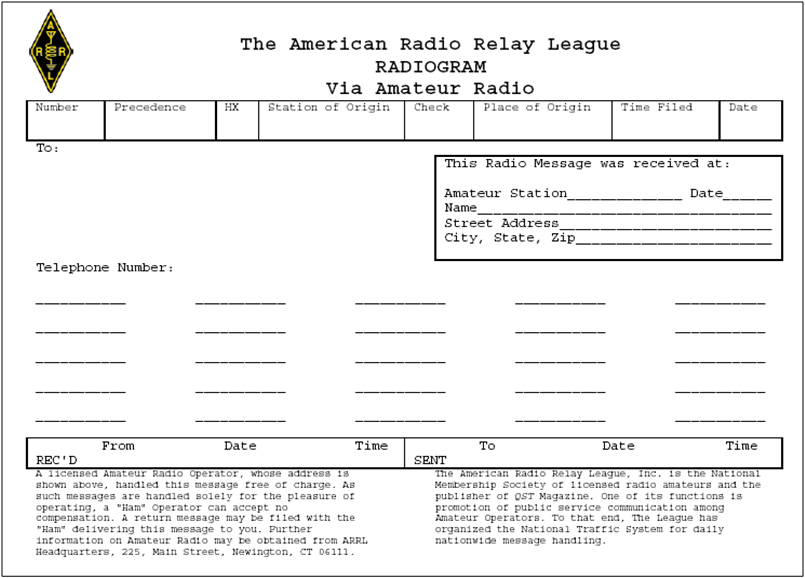
\includegraphics[width=\textwidth]{radiogramform.png}
\end{frame}

\section{Radio Speak}
\begin{frame}
\frametitle{Types of radio short-hand}
Amateur radio has its own codes, and slang. Much like 1337 or txt, this "shared language" makes it easier to communicate quickly, and efficently. Much of it comes from the days of telegraph and Morse Code.
\begin{description}
\item[Q Codes] - Three letter codes beginning with Q
\item[Number codes] - Codes sent as numbers, we really only us 73
\item[Pro-words] - Standardized ways of saying things in a clear and concise fashion
\item[Phonetics] - Words for letters, try saying BCDEZGT five times fast.
\end{description}
\end{frame}

\begin{frame}
\frametitle{Q-Codes}
Q codes are three letter codes that begin with Q and not QU and can be sent as either a question or a response. Really useful when using Morse Code as the codes are much shorter than what they represent. Some common Q codes are listed below.
\begin{description}
\item[QSY] Change frequency
\item[QRT] Stop transmitting
\item[QRZ] I'm calling
\item[QR\textbf<2->{M}] \textbf<2->{M}an made interference
\item[QR\textbf<2->{N}] \textbf<2->{N}atural interference or \textbf<2->{N}oise
\item[QSL] Acknowledge
\item[QST] Message to all amateurs
\end{description}
\end{frame}

\begin{frame}
\frametitle{Pro-words}
Pro or Professional words are used as shorthand, and because they prevent confusion. Yea and Nah kinda sound the same.
\begin{description}
\item[Roger] Received
\item[WilCO] Will Comply
\item[Over] I'm done talking for now
\item[Out] I'm done talking to you
\item[This Is] I'm going to say my callsign now
\item[Wait] Hold on for a while
\item[Affirmative] Yes
\item[Negative] No
\end{description}
\end{frame}

\begin{frame}
\frametitle{Phonetics}
In amateur radio we use ITU phonetics, this helps us reduce the potential of confusion over letters that sound the same
\begin{tabular}{l l l}
\scriptsize A - Alfa "AL-FAH"& \scriptsize  N - November "NO-VEM-BER" & \scriptsize  0 "ZEE-RO"\\
\scriptsize B - Bravo "BRAH-VOH"& \scriptsize  O - Oscar "OSS-CAH" & \scriptsize  1 "WUN"\\
\scriptsize C - Charlie "CHAR-LEE"& \scriptsize  P - Papa "PAH-PAH" & \scriptsize  2 "TOO"\\
\scriptsize D - Delta "DELL-TAH"& \scriptsize  Q - Quebec "KEH-BECK" & \scriptsize  3 "TH-UH-REE"\\
\scriptsize E - Echo "ECK-OH"& \scriptsize  R - Romeo "ROW-ME-OH & \scriptsize  4 "FOW-ER"\\
\scriptsize F - Foxtrot "FOKS-TROT"& \scriptsize  S - Sierra "SEE-AIR-RAH" & \scriptsize  5 "FI-IV" OR "FIFE"\\
\scriptsize G - Golf "GOLF"& \scriptsize  T - Tango "TANG-GO" & \scriptsize  6 "SIX"\\
\scriptsize H - Hotel "HOH-TELL"& \scriptsize  U - Uniform "YOU-NEE-FORM" & \scriptsize  7 "SEV-EN"\\
\scriptsize I - India "IN-DEE-AH"& \scriptsize  V - Victor "VIK-TAH" & \scriptsize  8 "ATE"\\
\scriptsize J - Juliett "JEW-LEE-ETT& \scriptsize  W - Whiskey "WISS-KEY" & \scriptsize  9 "NIN-ER"\\
\scriptsize K - Kilo "KEE-LOH"& \scriptsize  X - X-Ray "ECKS-RAY"\\
\scriptsize L - Lima "LEE-MAH& \scriptsize  Y - Yankee "YANG-KEY"\\
\scriptsize M - Mike "MIKE"& \scriptsize  Z - Zulu "ZOO-LOO"\\
\end{tabular}
W7QH becomes "Whiskey 7 Quebec Hotel" 
\end{frame}

\begin{frame}
\frametitle{CQ and 73}
There are two other special cases.
\begin{itemize}
\item CQ is the standard calling call. Think of it as Seek You, though no one really knows where it comes from. It is common to add extra stuff depending on the situation. You might hear CQ JOTA, CQ Field Day, CQ Contest, CQ DX, CQ Oregon. This lets people pick who they are looking for. A common general CQ would sound like "CQ CQ CQ this is KE7OSN calling CQ CQ CQ"
\item The other thing that comes up is the number 73, this goes back to the old Western Union Telegraph 92 codes, these were numbers that could be used in place of certain phrases, most of them dealing with packages or trains. 73 means "Beast Regards" and is generally used as "goodbye"
\end{itemize}
\end{frame}

\section{Other Practices}

\begin{frame}
\frametitle{Power}
In most amateur bands the maximum legal limit for power output is 1500 Watts, PEP. PEP - Peak Envelope Power is the largest amplitude of a signal. On some bands the limit is lower, for each band there is also a point at which you have to do a safety evaluation of your station to avoid unsafe exposure. You should always use the minimal power required to do what you need to do.
\end{frame}

\section{T2 Questions}
\subsection{T2A}
\begin{frame}
\frametitle{T2A 3 quesions from T2}
\begin{itemize}[<+->]
\tiny
\item\textbf{T2A01 What is the most common repeater frequency offset in the 2 meter band?}\\ B. plus or minus 600 kHz
\item\textbf{T2A02 What is the national calling frequency for FM simplex operations in the 70 cm band?}\\ D. 446.000 MHz
\item\textbf{T2A03 What is a common repeater frequency offset in the 70 cm band?}\\ A. Plus or minus 5 MHz
\item\textbf{T2A04 What is an appropriate way to call another station on a repeater if you know the other station's call sign?}\\ B. Say the station's call sign then identify with your call sign
\item\textbf{T2A05 What should you transmit when responding to a call of CQ?}\\ C. The other station's call sign followed by your call sign
\item\textbf{T2A06 What must an amateur operator do when making on-air transmissions to test equipment or antennas?}\\ A. Properly identify the transmitting station
\item\textbf{T2A07 Which of the following is true when making a test transmission?}\\ D. Station identification is required at least every ten minutes during the test and at the end
\item\textbf{T2A08 What is the meaning of the procedural signal "CQ"?}\\ D. Calling any station
\item\textbf{T2A09 What brief statement is often used in place of "CQ" to indicate that you are listening on a repeater?}\\ B. Say your call sign
\item\textbf{T2A10 What is a band plan, beyond the privileges established by the FCC?}\\ A. A voluntary guideline for using different modes or activities within an amateur band
\item\textbf{T2A11 What are the FCC rules regarding power levels used in the amateur bands?}\\ D. An amateur must use the minimum transmitter power necessary to carry out the desired communication
\end{itemize}
\tiny 79 of 396 19.9\%
\end{frame}

\subsection{T2B}
\begin{frame}
\frametitle{T2B 3 quesions from T2}
\begin{itemize}[<+->]
\tiny
\item\textbf{T2B01 What is the term used to describe an amateur station that is transmitting and receiving on the same frequency?}\\ C. Simplex communication
\item\textbf{T2B02 What is the term used to describe the use of a sub-audible tone transmitted with normal voice audio to open the squelch of a receiver?}\\ D. CTCSS
\item\textbf{T2B03 Which of the following describes the muting of receiver audio controlled solely by the presence or absence of an RF signal?}\\ B. Carrier squelch
\item\textbf{T2B04 Which of the following common problems might cause you to be able to hear but not access a repeater even when transmitting with the proper offset?}\\ A. The repeater receiver requires audio tone burst for access\\B. The repeater receiver requires a CTCSS tone for access\\C. The repeater receiver may require a DCS tone sequence for access\\D. All of these choices are correct
\item\textbf{T2B05 What determines the amount of deviation of an FM signal?}\\ C. The amplitude of the modulating signal
\item\textbf{T2B06 What happens when the deviation of an FM transmitter is increased?}\\ A. Its signal occupies more bandwidth
\item\textbf{T2B07 What should you do if you receive a report that your station s transmissions are causing splatter or interference on nearby frequencies?}\\ D. Check your transmitter for off-frequency operation or spurious emissions
\item\textbf{T2B08 What is the proper course of action if your station s transmission unintentionally interferes with another station?}\\ B. Properly identify your transmission and move to a different frequency
\item\textbf{T2B09 Which of the following methods is encouraged by the FCC when identifying your station when using phone?}\\ A. Use of a phonetic alphabet
\item\textbf{T2B10 What is the "Q" signal used to indicate that you are receiving interference from other stations?}\\ A. QRM
\item\textbf{T2B11 What is the "Q" signal used to indicate that you are changing frequency?}\\ B. QSY
\end{itemize}
\tiny 90 of 396 22.7\%
\end{frame}

\subsection{T2C}
\begin{frame}
\frametitle{T2C 3 quesions from T2}
\begin{itemize}[<+->]
\tiny
\item\textbf{T2C01 What set of rules applies to proper operation of your station when using amateur radio at the request of public service officials?}\\ C. FCC Rules
\item\textbf{T2C04 What do RACES and ARES have in common?}\\ D. Both organizations may provide communications during emergencies
\item\textbf{T2C05 What is the Radio Amateur Civil Emergency Service?}\\ B. A radio service using amateur stations for emergency management or civil defense communications
\item\textbf{T2C06 Which of the following is common practice during net operations to get the immediate attention of the net control station when reporting an emergency?}\\ C. Begin your transmission with  Priority  or  Emergency  followed by your call sign
\item\textbf{T2C07 What should you do to minimize disruptions to an emergency traffic net once you have checked in?}\\ C. Do not transmit on the net frequency until asked to do so by the net control station
\item\textbf{T2C08 What is usually considered to be the most important job of an amateur operator when handling emergency traffic messages?}\\ A. Passing messages exactly as written, spoken or as received
\item\textbf{T2C09 When may an amateur station use any means of radio communications at its disposal for essential communications in connection with immediate safety of human life and protection of property?}\\ B. When normal communications systems are not available
\item\textbf{T2C10 What is the preamble in a formal traffic message?}\\ D. The information needed to track the message as it passes through the amateur radio traffic handling system
\item\textbf{T2C11 What is meant by the term "check" in reference to a formal traffic message?}\\ A. The check is a count of the number of words or word equivalents in the text portion of the message
\end{itemize}
\tiny 101 of 396 25.5\%
\end{frame}

\part{Radio wave characteristics, radio and electromagnetic properties, propagation modes}
\section{Electromagnetic Waves}
\begin{frame}
\frametitle{Electromagnetic Waves}
Electromagnetic waves are energy waves that move through space, similar to the way waves move in water or sound through air.\\
In a vacuum these waves move at the speed of light 299,792,458$m/s$ or 186,282.397$miles/second$. This is good as these waves are light.
\end{frame}

\begin{frame}
\frametitle{Speed of light}
We can round up to 300,000,000$m/s$. Some distance measured in terms of light-time
\begin{description}
\item[Average distance between the Sun and Earth] - 8 minutes
\item[GEO Satellite to Earth's Surface] - about a half second
\item[Nearest other star to our Sun] 4.25 Years
\item[Voyager Space probe to the Sun] at 18,884,401,200 Km from the sun? \only<2->{$\frac{\frac{18884401200Km}{300000Km/s}}{3600s}=Hours$} \only<3->{17:08:00-ish}
\end{description}
\end{frame}

\begin{frame}
\frametitle{Frequency - not just an ok movie}
We often refer to a wave by it's frequency. Frequency is the number of times a wave cycles in a given time. We use Hertz (Hz) which has the unites of $\frac{1}{Seconds}$.\\
Middle C is 440Hz, or 440 cycles per second.\\
KLOO-AM is 1.340MHz, or 1,340,000 cycles per second.
\end{frame}

\begin{frame}
\frametitle{SI Prefixs}
Sometimes it is a lot easier to shorten things up a bit.
\begin{description}
\item[Tera]T $10^{12}$ 1,000,000,000,000
\item[Giga]G $10^9$ 1,000,000,000
\item[Mega]M $10^6$ 1,000,000
\item[Kilo]K $10^3$ 1,000
\item[Deci]d $10^{-1}$ 0.1
\item[Ceni]c $10^{-2}$ 0.01
\item[Milli]m $10^{-3}$ 0.001
\item[Micro]$\mu$ $10^{-6}$ 0.000001
\item[Nano]n $10^{-9}$ 0.000000001
\item[Pico]p $10^{-12}$ 0.000000000001
\end{description}
\end{frame}

\begin{frame}
\frametitle{Wavelength}
We also use wavelength to describe waves. The wavelength is the distance between two like points on the wave exactly one cycle apart, e.g.\ the distance between peaks.\\
\begin{center}
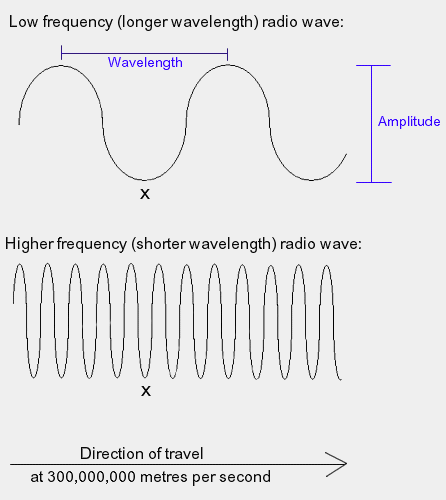
\includegraphics[width=0.85\textwidth,height=0.7\textheight]{wavelength.png}
\end{center}
\end{frame}

\begin{frame}
\frametitle{ElectoMagnetic}
\begin{center}
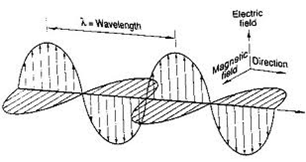
\includegraphics[height=0.5\textheight]{emwave.png}\\
\end{center}
Electromagnetic waves have two parts, one electric part, and one magnetic part. The magnetic part is rotated and phase shifted by 90$^{\circ}$
\end{frame}

\begin{frame}
\frametitle{Wavelength to frequency and back}
It is easy to convert between wavelength and frequency just use the equation below.\\
\only<2->{$Wavelength(meters) = \frac{300}{Freq. (MHz)}$\\}
\only<3->{We'll practice on the next slide}
\end{frame}

\begin{frame}
\frametitle{MATH!!!}
\begin{itemize}
\item Lets try to convert 7.025MHz into a wavelength to figure out which band it belongs to.\\
\only<2->{$Wavelength(\lambda)=\frac{300}{7.025}$} \only<3->{that comes out to 42.7meters\\}
\only<4->{That fits nicely in the 40meter band\\}
\item<5-> Now lets try 223.50MHz\\
$\frac{300}{223.50}=?$ \only<6->{1.35, for the 1.25meter band.}
\end{itemize}
\end{frame}

\section{Propagation}
\begin{frame}
\frametitle{Line of sight}
Just like light radio waves travel in a straight line.\\
\only<2->{They also reflect off some things like light.\\}
\only<3->{If there are multiple ways for radio waves to get between two points we call this Multipath, and it creates interference.\\}
\only<4->{Reflections can be really useful when you don't have a direct line of sight.\\}
\only<5->{Radio waves will also refract.\\}
\end{frame}

\begin{frame}
\frametitle{Solar Wind}
\begin{center}
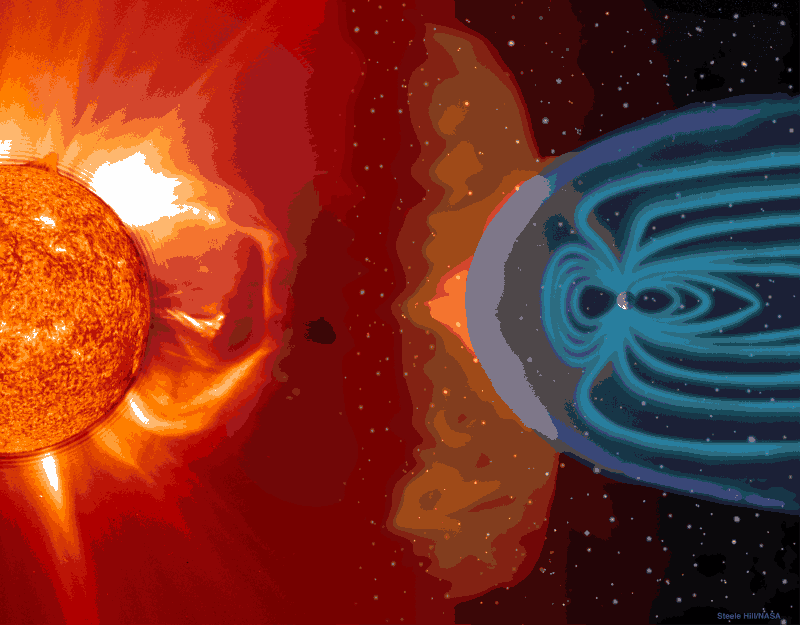
\includegraphics[width=\textwidth]{magfield.png}
\end{center}
\end{frame}

\begin{frame}
\frametitle{Solar Radiation}
Solar radiation charges atoms in the atmosphere, breaking loose electrons, to create ions, which can interact with radio waves.\\
\begin{columns}
\column{.3\textwidth}
At night the electrons recombined with their atoms. This means things change from day to night.
\column{.7\textwidth}
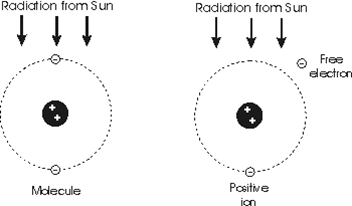
\includegraphics[width=\textwidth]{ions.png}
\end{columns}
\end{frame}

\begin{frame}
\frametitle{Ionosphere}
\begin{columns}
\column{.6\textwidth}
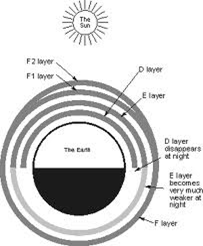
\includegraphics[height=.9\textheight]{ionosphere.png}
\column{.4\textwidth}
The parts of the atmosphere most affected by ionization are collectively called the Ionosphere!\\
It has multiple layers, each interact differently with radio waves. The D layers mostly absorbs RF, while the E and F layers reflect.\\
HF is is ruled by the ionosphere\\ VHF and up \ldots not so much.
\end{columns}
\end{frame}

\begin{frame}
\frametitle{Ionosphere}
During the day the D layers absorbs a large chunk of HF, at night it goes away and signals bounce (refract) off the E and F layers.\\
VHF and above mostly just goes through the ionosphere\ldots\\
But sometimes at night there is just enough E layer to refract VHF signals. We call this "Sporadic E"
\end{frame}

\begin{frame}
\frametitle{Auroras and Meteor Showers}
The auroras are a visible sign of ionization, as they move they can cause received signals to sound fluttery.\\
Meteor showers leave short lived trails of ionized gases, that can refract signals, these effects are impossible to predict and last seconds.\\
You can even bounce radio signals off the moon!
\end{frame}

\begin{frame}
\frametitle{Tropospheric Ducting}
\begin{center}
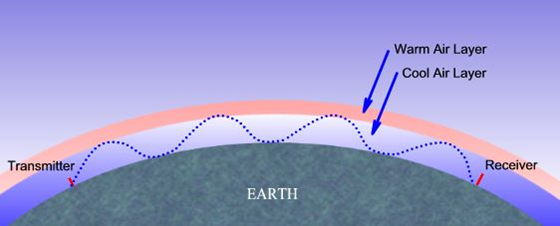
\includegraphics[width=\textwidth]{troposhpere.png}
\end{center}
Air can refract electromagnetic radiation. A temperature inversion (warm air above cold) can cause VHF signals to refract and travel long distances.\\
This is called "Tropospheric Ducting" and often happens between here and Hawaii, it mostly affects VHF.
\end{frame}

\begin{frame}
\frametitle{Knife Edge}
\begin{center}
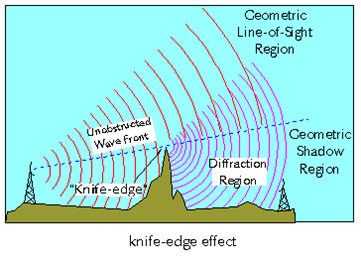
\includegraphics[height=.9\textheight]{knifeedge.png}
\end{center}
\end{frame}

\begin{frame}
\frametitle{Polarization}
Antennas tend to radiate and receive waves polarized along the direction of the antenna. An antenna pointing vertically produces vertically polarized waves, and the equivalent is true for a horizontal antenna.\\
If the polarization of the receiving antenna does not match the wave it is receiving then the signal strength is reduced by a significant degree. In an ideal world without the magnetic portion of a wave two antennas rotated $\pm90^{\circ}$ would not be able to "see" each other.
\end{frame}
\section{T3 Questions}
\subsection{T3A}
\begin{frame}
\frametitle{Title}
\begin{itemize}[<+->]
\tiny
\item\textbf{T3A01 What should you do if another operator reports that your station s 2 meter signals were strong just a moment ago, but now they are weak or distorted?}\\ D. Try moving a few feet, as random reflections may be causing multi-path distortion
\item\textbf{T3A02 (B) Why are UHF signals often more effective from inside buildings than VHF signals?}\\ B. The shorter wavelength allows them to more easily penetrate the structure of buildings
\item\textbf{T3A03 What antenna polarization is normally used for long-distance weak-signal CW and SSB contacts using the VHF and UHF bands?}\\ C. Horizontal
\item\textbf{T3A04 What can happen if the antennas at opposite ends of a VHF or UHF line of sight radio link are not using the same polarization?}\\ B. Signals could be significantly weaker
\item\textbf{T3A05 When using a directional antenna, how might your station be able to access a distant repeater if buildings or obstructions are blocking the direct line of sight path?}\\ B. Try to find a path that reflects signals to the repeater
\item\textbf{T3A06 What term is commonly used to describe the rapid fluttering sound sometimes heard from mobile stations that are moving while transmitting?}\\ B. Picket fencing
\item\textbf{T3A07 What type of wave carries radio signals between transmitting and receiving stations?}\\ A. Electromagnetic
\item\textbf{T3A08 What is the cause of irregular fading of signals from distant stations during times of generally good reception?}\\ C. Random combining of signals arriving via different path lengths
\item\textbf{T3A09 Which of the following is a common effect of "skip" reflections between the Earth and the ionosphere?}\\ B. The polarization of the original signal is randomized
\item\textbf{T3A10 What may occur if VHF or UHF data signals propagate over multiple paths?}\\ D. Error rates are likely to increase
\item\textbf{T3A11 Which part of the atmosphere enables the propagation of radio signals around the world?}\\ C. The ionosphere
\end{itemize}
\tiny 112 of 396 28.3\%
\end{frame}

\subsection{T3B}
\begin{frame}
\frametitle{Title}
\begin{itemize}[<+->]
\tiny
\item\textbf{T3B01 What is the name for the distance a radio wave travels during one complete cycle?}\\ C. Wavelength
\item\textbf{T3B02 What term describes the number of times per second that an alternating current reverses direction?}\\ D. Frequency
\item\textbf{T3B03 What are the two components of a radio wave?}\\ C. Electric and magnetic fields
\item\textbf{T3B04 How fast does a radio wave travel through free space?}\\ A. At the speed of light
\item\textbf{T3B05 How does the wavelength of a radio wave relate to its frequency?}\\ B. The wavelength gets shorter as the frequency increases
\item\textbf{T3B06 What is the formula for converting frequency to wavelength in meters?}\\ D. Wavelength in meters equals 300 divided by frequency in megahertz
\item\textbf{T3B07 What property of radio waves is often used to identify the different frequency bands?}\\ A. The approximate wavelength
\item\textbf{T3B08 What are the frequency limits of the VHF spectrum?}\\ B. 30 to 300 MHz
\item\textbf{T3B09 What are the frequency limits of the UHF spectrum?}\\ D. 300 to 3000 MHz
\item\textbf{T3B10 What frequency range is referred to as HF?}\\ C. 3 to 30 MHz
\item\textbf{T3B11 What is the approximate velocity of a radio wave as it travels through free space?}\\ B. 300,000,000 meters per second
\end{itemize}
\tiny 123 of 396 31.0\%
\end{frame}

\subsection{T3C}
\begin{frame}
\frametitle{Title}
\begin{itemize}[<+->]
\tiny
\item\textbf{T3C01 Why are "direct" (not via a repeater) UHF signals rarely heard from stations outside your local coverage area?}\\ C. UHF signals are usually not reflected by the ionosphere
\item\textbf{T3C02 Which of the following might be happening when VHF signals are being received from long distances?}\\ D. Signals are being refracted from a sporadic E layer
\item\textbf{T3C03 What is a characteristic of VHF signals received via auroral reflection?}\\ B. The signals exhibit rapid fluctuations of strength and often sound distorted
\item\textbf{T3C04 Which of the following propagation types is most commonly associated with occasional strong over-the-horizon signals on the 10, 6, and 2 meter bands?}\\ B. Sporadic E
\item\textbf{T3C05 What is meant by the term "knife-edge" propagation?}\\ C. Signals are partially refracted around solid objects exhibiting sharp edges
\item\textbf{T3C06 What mode is responsible for allowing over-the-horizon VHF and UHF communications to ranges of approximately 300 miles on a regular basis?}\\ A. Tropospheric scatter
\item\textbf{T3C07 What band is best suited to communicating via meteor scatter?}\\ B. 6 meters
\item\textbf{T3C08 What causes "tropospheric ducting"?}\\ D. Temperature inversions in the atmosphere
\item\textbf{T3C09 What is generally the best time for long-distance 10 meter band propagation?}\\ A. During daylight hours
\item\textbf{T3C10 What is the radio horizon?}\\ A. The distance at which radio signals between two points are effectively blocked by the curvature of the Earth
\item\textbf{T3C11 Why do VHF and UHF radio signals usually travel somewhat farther than the visual line of sight distance between two stations?}\\ C. The Earth seems less curved to radio waves than to light
\end{itemize}
\tiny 134 of 396 33.8\%
\end{frame}

\part{Amateur radio practices and station set up}
\begin{frame}
\frametitle{Technician class section 4}
This section is going to be really short as much of the details fit in better elsewhere
\end{frame}
\section{Station setup; microphone, speaker, headphones, filters, power source, connecting a computer, RF grounding}
\begin{frame}
\frametitle{Station setup; microphone, speaker, headphones, filters, power source, connecting a computer, RF grounding}
Some microphones include push-to-talk and voltage connections. Headphones can be useful in a noisy area instead of a speaker. A regulated power supply reduces voltage fluctuations. Filters between the transmitter and antenna can reduce harmonic emissions. A band-reject filter is a good first step if your 2 meter radio is causing problems with a TV. A terminal node controller is a modem for your radio, your soundcard can be a modem too. Flat straps are good grounding cables. Ferrite chokes can reduce RF current in cables. If your radio whines in your car and it goes along with the engine its probably the alternator. A radio installed in a car should be connected to a good "ground"
\end{frame}

\section{Operating controls; tuning, use of filters, squelch, AGC, repeater offset, memory channels}
\begin{frame}
\frametitle{Operating controls; tuning, use of filters, squelch, AGC, repeater offset, memory channels}
If your mic is turned up to loud your signal may distort. You can set the frequency of a radio with the keypad or VFO knob. Squelch lets you mute the receiver when no signal is coming in. You can program favorite frequencies in memory. The noise blanker option can reduce noise. The RIT or Receiver Incremental Tuning control can change the pitch of the received audio. A good filter setting for SSB is 2400Hz, and 500Hz for CW. A repeater offset is the difference in its receive and transmit frequencies.
\end{frame}

\section{T4 Questions}
\subsection{T4A}
\begin{frame}
\frametitle{T4A questions}
\begin{itemize}[<+->]
\tiny
\item\textbf{TA01 (B) Which of the following is true concerning the microphone connectors on amateur transceivers?}\\ B. Some connectors include push-to-talk and voltages for powering the microphone
\item\textbf{T4A02 (C) What could be used in place of a regular speaker to help you copy signals in a noisy area?}\\ C. A set of headphones
\item\textbf{T4A03 (A) Which is a good reason to use a regulated power supply for communications equipment?}\\ A. It prevents voltage fluctuations from reaching sensitive circuits
\item\textbf{T4A04 (A) Where must a filter be installed to reduce harmonic emissions?}\\ A. Between the transmitter and the antenna
\item\textbf{T4A05 (D) What type of filter should be connected to a TV receiver as the first step in trying to prevent RF overload from a nearby 2 meter transmitter?}\\ D. Band-reject filter
\item\textbf{T4A06 (C) Which of the following would be connected between a transceiver and computer in a packet radio station?}\\ C. Terminal node controller
\item\textbf{T4A07 (C) How is the computer s sound card used when conducting digital communications using a computer?}\\ C. The sound card provides audio to the microphone input and converts received audio to digital form
\item\textbf{T4A08 (D) Which type of conductor is best to use for RF grounding?}\\ D. Flat strap
\item\textbf{T4A09 (D) Which would you use to reduce RF current flowing on the shield of an audio cable?}\\ D. Ferrite choke
\item\textbf{T4A10 (B) What is the source of a high-pitched whine that varies with engine speed in a mobile transceiver s receive audio?}\\ B. The alternator
\item\textbf{T4A11 (A) Where should a mobile transceiver's power negative connection be made?}\\ A. At the battery or engine block ground strap
\end{itemize}
\tiny 145 of 396  36.6\%
\end{frame}

\subsection{T4B}
\begin{frame}
\frametitle{T 4B questions}
\begin{itemize}[<+->]
\tiny
\item\textbf{T4B01 (B) What may happen if a transmitter is operated with the microphone gain set too high?}\\ B. The output signal might become distorted
\item\textbf{T4B02 (A) Which of the following can be used to enter the operating frequency on a modern transceiver?}\\ A. The keypad or VFO knob
\item\textbf{T4B03 (D) What is the purpose of the squelch control on a transceiver?}\\ D. To mute receiver output noise when no signal is being received
\item\textbf{T4B04 (B) What is a way to enable quick access to a favorite frequency on your transceiver?}\\ B. Store the frequency in a memory channel
\item\textbf{T4B05 (C) Which of the following would reduce ignition interference to a receiver?}\\ C. Turn on the noise blanker
\item\textbf{T4B06 (D) Which of the following controls could be used if the voice pitch of a single-sideband signal seems too high or low?}\\ D. The receiver RIT or clarifier
\item\textbf{T4B07 (B) What does the term "RIT" mean?}\\ B. Receiver Incremental Tuning
\item\textbf{T4B08 (B) What is the advantage of having multiple receive bandwidth choices on a multimode transceiver?}\\ B. Permits noise or interference reduction by selecting a bandwidth matching the mode
\item\textbf{T4B09 (C) Which of the following is an appropriate receive filter to select in order to minimize noise and interference for SSB reception?}\\ C. 2400 Hz
\item\textbf{T4B10 (A) Which of the following is an appropriate receive filter to select in order to minimize noise and interference for CW reception?}\\ A. 500 Hz
\item\textbf{T4B11 (C) Which of the following describes the common meaning of the term  repeater offset ?}\\ C. The difference between the repeater s transmit and receive frequencies
\end{itemize}
\tiny 156 of 396  39.4\%
\end{frame}

\part{Electrical principles, math for electronics, electronic principles, Ohm s Law}
\section{Ohm's Law}
\begin{frame}
\frametitle{Ohm, Ohm on the range}
Most metals are good at conducting electricity, this means they allow electrons to move around. We make wires that allow us to move electrons from one specific place to another.
\end{frame}
\subsection{Current}
\begin{frame}
\frametitle{Current}
The movement of electrons is called \textbf{Current}. We measure current in the Ampere, aka the Amp, aka A (or I).\\
Current that moves in only one direction is called \textbf{Direct Current (DC)}. Current that changes direction regularly is called \textbf{Alternating Current (AC)}.\\
A device that measures current is an ammeter.
\end{frame}

\begin{frame}
\frametitle{Ideas of current}
\begin{center}

\includegraphics[height=.9\textheight]{acdc.jpg}<1>
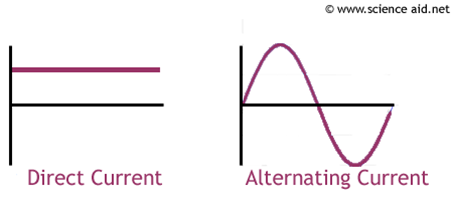
\includegraphics[width=\textwidth]{acdc.png}<2>
\end{center}
\end{frame}

\subsection{Voltage}
\begin{frame}
\frametitle{The Electromotive Force}
The force that causes electrons to flow is called \only{\ldots}<1>\pause \textbf{The Electromotive Force}.\\
 We measure this force as \only{\ldots}<2>\pause\textbf{ Voltage}, or \textbf{V}.\\
Voltage is measured with a \only{\ldots}<3>\pause \textbf{Voltmeter}
\end{frame}

\begin{frame}
\frametitle{Voltage}
Electrons like to spread out. It's their "natural desire" to not get bunched up that causes voltage. There can be voltage without current, but not current without voltage.\\
An unconnected battery has a voltage, but until it is hooked up to a complete circuit the electrons can't go anywhere.\\
Voltage is the difference in electrical potential between two points. Think of something falling down stairs.
\end{frame}

\subsection{Resistance}

\begin{frame}
\frametitle{The Resistor}
Resistance, impedes the flow of electrons.\\
The unit of resistance is the Ohm, or $\Omega$. \pause If that looks Greek, that's because it is, that Omega, a letter from the Greek alphabet\\ \only<3>{Now sing along \ldots \\ Alpha $A$, Beta $B$, Gamma $\Gamma$, Delta $\Delta$, Epsilon $E$, Zeta $Z$, Eta $H$, Theta $\Theta$, Iota $I$. \\Anyone? } \only{Resistance is measured with an ohmmeter.\\ Never use an ohmmeter on a live circuit}<4->
\begin{center}
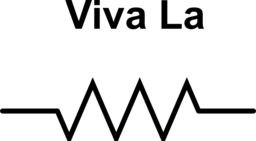
\includegraphics[width=.25\textwidth]{viva.png}<4->
\end{center}
\end{frame}

\subsection{Ohms Law}
\begin{frame}
\frametitle{Ohms Law}
The voltage across a resistor is equal to the resistance times the current. $V=IR$.\\
If we take a 9volt battery and connect it to a 90$\Omega$ resistor, what is the current through it?\pause\\
$V=IR\to I=\frac{V}{R}\to I=\frac{9}{90}$\pause$\to 0.1=\frac{9}{90}$ 0.1 Amps, or 100 milliamps.
\end{frame}

\begin{frame}
\frametitle{Power}
When current flows through an impedance it dissipates energy as "POWER". Power is measured Watts (W).\\
The equation for power is $P=IV$\pause Lets try with our prior example, we had 9volts and .1amps.\\
$P=IV \to P=9*.1$\pause$\to 0.9=9*.1$
\end{frame}

\section{Components}
\begin{frame}
\frametitle{Electrical Components}
\begin{center}
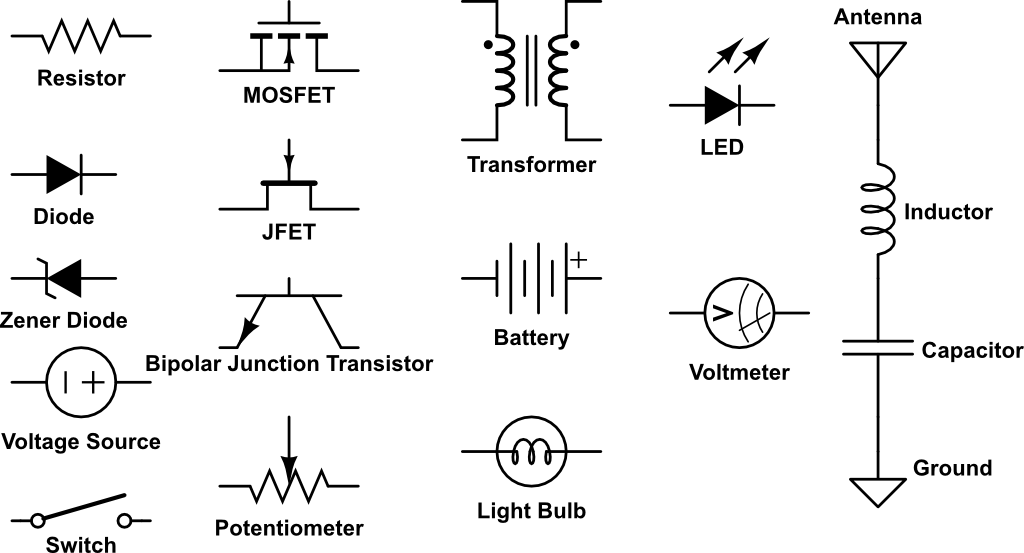
\includegraphics[width=\textwidth]{components.png}
\end{center}
\end{frame}

\subsection{The Resistor}
\begin{frame}
\frametitle{The Resistor}
Resistors are the electrical component that provides resistance. On paper they are squiggly lines, in real life they look like.\\\pause
\begin{center}
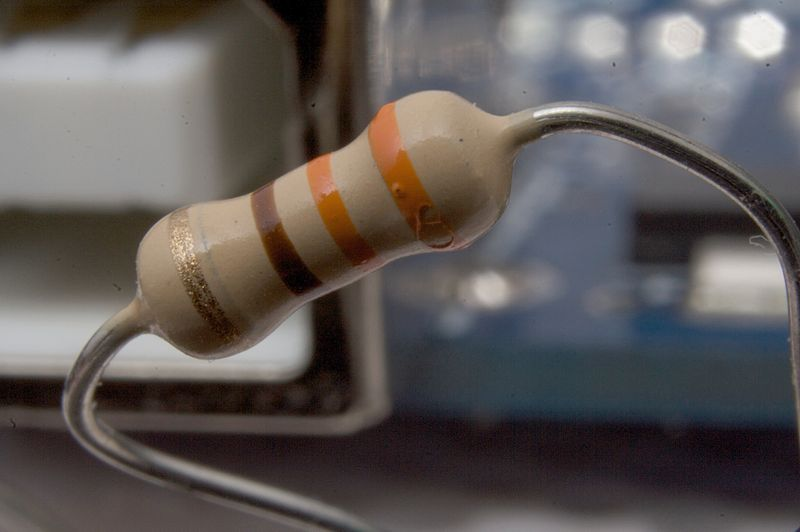
\includegraphics[height=.8\textheight]{resistor.jpg}
\end{center}
\end{frame}

\subsection{The Capacitor}
\begin{frame}
\frametitle{The Capacitor}
Capacitors store energy in an electrostatic field. They are made of two conducting plates separated by an insulated material. electrons build up on one plate when charged. They pass AC fairly well, but can block DC. They are represented as two parallel lines, one may be curved. There are three types, a normal type that can be reversed, an electrolytic type that is polarized (they have a + or a - to note which way the go), and variable ones with an arrow through them.\\\pause
\begin{center}
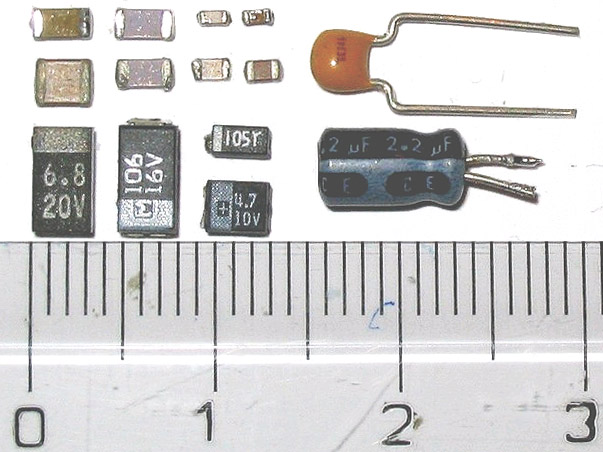
\includegraphics[height=.5\textheight]{capacitor.jpg}
\end{center}
\end{frame}

\begin{frame}
\frametitle{Warning}
\begin{center}
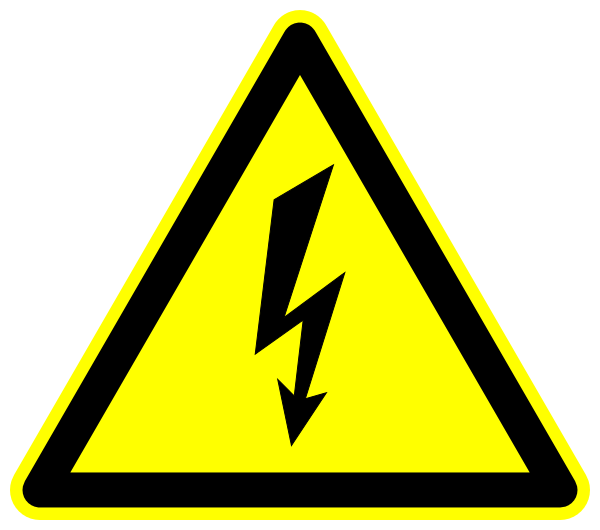
\includegraphics[height=.5\textheight]{shockhazard.png}
\end{center}
Capacitors can store a charge for some time. They can shock with ease, at best it will hurt, at worst it can cause burns and even stop your heart.
\end{frame}

\subsection{The Inductor}

\begin{frame}
\frametitle{The Inductor}
Inductors pass current in DC circuits, and impedes AC. They store energy in a magnetic field, magnetic fields require energy to change. This means that \textbf{any} change in current. The unit of inductance is the Henry.\\
They are made by winding wire in a coil. The more winds the more inductance. Sometimes iron is inserted in the middle to increase the inductance.
\begin{center}
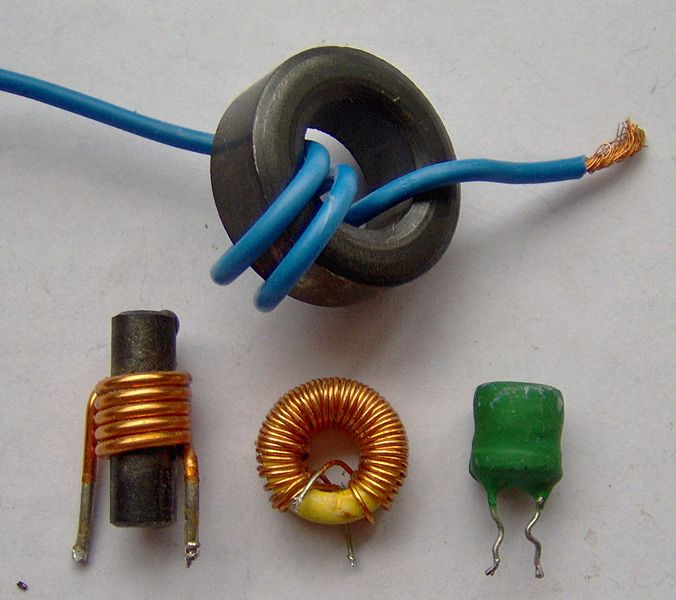
\includegraphics[height=.4\textheight]{inductor.jpg}
\end{center}

\end{frame}

\begin{frame}
\frametitle{More Inductance}
\begin{center}
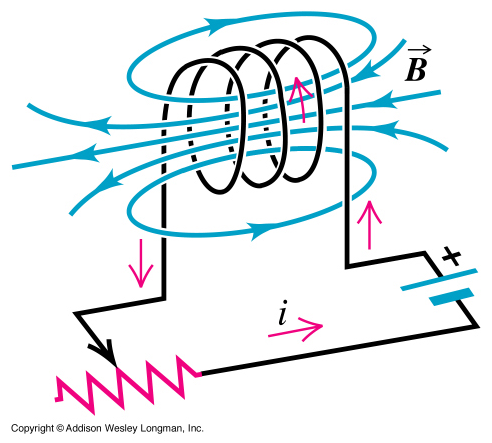
\includegraphics[height=.9\textheight]{inductor.png}
\end{center}
\end{frame}

\subsection{Relay}
\begin{frame}
\frametitle{Relays}
An inductor next to a magnetic switch creates a relay. They can be used to separate high current, or voltage circuits from low ones.
\end{frame}

\subsection{Diode}
\begin{frame}
\frametitle{Diodes}
Diodes prevent current from moving in one direction, while doing not much to current in the other. Some of them give off light. Others known as Zener diodes will let current flow against them if the voltage is high enough.\\
\begin{center}
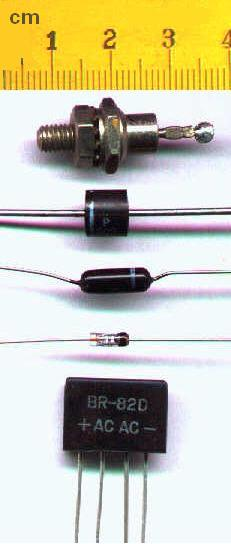
\includegraphics[angle=90,width=\textwidth]{diode.jpg}
\end{center}
\end{frame}

\subsection{Transistors}
\begin{frame}
\frametitle{Transistors}
Transistors allow a small current to control a much larger one. This gives transistors "gain". Two types we care about are Bi-polar Junction (BJT), and Field Effect (FET).
\end{frame}

\begin{frame}
\frametitle{BJT's}
Bipolar Junction Transistors come in two types, NPN and PNP. Both have three connections, an emitter, a collector, and a base. In diagrams the emitter is the wire with an arrow, the collector is on the same "side" as the emitter, and the base goes out the other way, if you turn it so it would stand on the two legs the base is the top. With an NPN current is allowed to flow from the collector to the emitter when there is enough voltage between the emitter and the base. in NPN's the arrow \textbf{N}ever \textbf{P}oints i\textbf{N}.\\PNP's allow current to flow from the emitter to the collector when there is enough voltage between the emitter and the base. For PNP's the arrow \textbf{P}oints i\textbf{N} \textbf{P}ermanently\\
\begin{center}
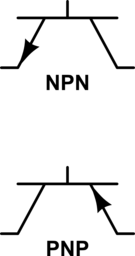
\includegraphics{bjts.png}
\end{center}
\end{frame}

\begin{frame}
\frametitle{MOSFET's}
Metal Oxide Semiconductor Field Effect Transistors work much like BJT's but they are a little different. In the diagrams if the arrow points out they are P-channel, and if it points i\textbf{N} its an N-channel. The three wires are a Gate, a Drain, and a Source. The wire with the arrow is the source, the drain is on the same side as the source, and the other one is the gate. In either case if there is a large enough voltage between the source and the gate current can flow in the direction of the arrow between the source and the drain.
\begin{center}
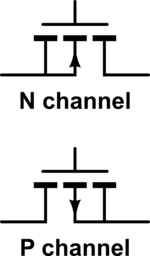
\includegraphics{mosfets.png}
\end{center}
\end{frame}

\subsection{Batteries}
\begin{frame}
\frametitle{Batteries}
Similar to capacitors batteries store electrical energy, however they store that energy via chemical reaction instead of an electric field. There are many different types of batteries. They fall into two categories; Primary, that can produce current as soon as they are made, and Secondary, that have to be charged first. There are also Dry cells and Wet cells. Common batteries are Alkaline, Li-Ion, NiCad, NiMH,ZiC, Lead-Acid. Each type has different properties, advantages and disadvantages.
\end{frame}

\section{T5 Questions}
\subsection{T5A}
\begin{frame}
\frametitle{T5A Questions}
\begin{itemize}[<+->]
\tiny
\item\textbf{T5A01 (D) Electrical current is measured in which of the following units?}\\D. Amperes
\item\textbf{T5A02 (B) Electrical power is measured in which of the following units?}\\B. Watts
\item\textbf{T5A03 (D) What is the name for the flow of electrons in an electric circuit?}\\D. Current
\item\textbf{T5A04 (B) What is the name for a current that flows only in one direction?}\\B. Direct current
\item\textbf{T5A05 (A) What is the electrical term for the electromotive force (EMF) that causes electron flow?}\\A. Voltage
\item\textbf{T5A06 (A) How much voltage does a mobile transceiver usually require?}\\A. About 12 volts
\item\textbf{T5A07 (C) Which of the following is a good electrical conductor?}\\C. Copper
\item\textbf{T5A08 (B) Which of the following is a good electrical insulator?}\\B. Glass
\item\textbf{T5A09 (A) What is the name for a current that reverses direction on a regular basis?}\\A. Alternating current
\item\textbf{T5A10 (C) Which term describes the rate at which electrical energy is used?}\\C. Power
\item\textbf{T5A11 (A) What is the basic unit of electromotive force?}\\A. The volt
\end{itemize}
\tiny 167 of 396  42.2\%
\end{frame}

\subsection{T5B}
\begin{frame}
\frametitle{T5B}
\tiny
\begin{itemize}[<+->]
\item\textbf{T5A01 (D) Electrical current is measured in which of the following units?}\\D. Amperes
\item\textbf{T5A02 (B) Electrical power is measured in which of the following units?}\\B. Watts
\item\textbf{T5A03 (D) What is the name for the flow of electrons in an electric circuit?}\\D. Current
\item\textbf{T5A04 (B) What is the name for a current that flows only in one direction?}\\B. Direct current
\item\textbf{T5A05 (A) What is the electrical term for the electromotive force (EMF) that causes electron flow?}\\A. Voltage
\item\textbf{T5A06 (A) How much voltage does a mobile transceiver usually require?}\\A. About 12 volts
\item\textbf{T5A07 (C) Which of the following is a good electrical conductor?}\\C. Copper
\item\textbf{T5A08 (B) Which of the following is a good electrical insulator?}\\B. Glass
\item\textbf{T5A09 (A) What is the name for a current that reverses direction on a regular basis?}\\A. Alternating current
\item\textbf{T5A10 (C) Which term describes the rate at which electrical energy is used?}\\C. Power
\item\textbf{T5A11 (A) What is the basic unit of electromotive force?}\\A. The volt
\end{itemize}
\tiny 178 of 396  44.9\%
\end{frame}

\subsection{T5C}
\begin{frame}
\frametitle{T5C}
\tiny
\begin{itemize}[<+->]
\item\textbf{T5C01 (D) What is the ability to store energy in an electric field called?}\\D. Capacitance
\item\textbf{T5C02 (A) What is the basic unit of capacitance?}\\A. The farad
\item\textbf{T5C03 (D) What is the ability to store energy in a magnetic field called?}\\D. Inductance
\item\textbf{T5C04 (C) What is the basic unit of inductance?}\\C. The henry
\item\textbf{T5C05 (A) What is the unit of frequency?}\\A. Hertz
\item\textbf{T5C06 (C) What is the abbreviation that refers to radio frequency signals of all types?}\\C. RF
\item\textbf{T5C07 (C) What is a usual name for electromagnetic waves that travel through space?}\\C. Radio waves
\item\textbf{T5C08 (A) What is the formula used to calculate electrical power in a DC circuit?}\\A. Power (P) equals voltage (E) multiplied by current (I)
\item\textbf{T5C09 (A) How much power is being used in a circuit when the applied voltage is 13.8 volts DC and the current is 10 amperes?}\\A. 138 watts
\item\textbf{T5C10 (B) How much power is being used in a circuit when the applied voltage is 12 volts DC and the current is 2.5 amperes?}\\B. 30 watts
\item\textbf{T5C11 (B) How many amperes are flowing in a circuit when the applied voltage is 12 volts DC and the load is 120 watts?}\\B. 10 amperes
\end{itemize}
\tiny 189 of 396  47.7\%
\end{frame}

\subsection{T5D}
\begin{frame}
\frametitle{T5D}
\tiny
\begin{itemize}[<+->]
\item\textbf{T5D01 (B) What formula is used to calculate current in a circuit?}\\B. Current (I) equals voltage (E) divided by resistance (R)
\item\textbf{T5D02 (A) What formula is used to calculate voltage in a circuit?}\\A. Voltage (E) equals current (I) multiplied by resistance (R)
\item\textbf{T5D03 (B) What formula is used to calculate resistance in a circuit?}\\B. Resistance (R) equals voltage (E) divided by current (I)
\item\textbf{T5D04 (B) What is the resistance of a circuit in which a current of 3 amperes flows through a resistor connected to 90 volts?}\\B. 30 ohms
\item\textbf{T5D05 (C) What is the resistance in a circuit for which the applied voltage is 12 volts and the current flow is 1.5 amperes?}\\C. 8 ohms
\item\textbf{T5D06 (A) What is the resistance of a circuit that draws 4 amperes from a 12-volt source?}\\A. 3 ohms
\item\textbf{T5D07 (D) What is the current flow in a circuit with an applied voltage of 120 volts and a resistance of 80 ohms?}\\D. 1.5 amperes
\item\textbf{T5D08 (C) What is the current flowing through a 100-ohm resistor connected across 200 volts?}\\C. 2 amperes
\item\textbf{T5D09 (C) What is the current flowing through a 24-ohm resistor connected across 240 volts?}\\C. 10 amperes
\item\textbf{T5D10 (A) What is the voltage across a 2-ohm resistor if a current of 0.5 amperes flows through it?}\\A. 1 volt
\item\textbf{T5D11 (B) What is the voltage across a 10-ohm resistor if a current of 1 ampere flows through it?}\\B. 10 volts
\item\textbf{T5D12 (D) What is the voltage across a 10-ohm resistor if a current of 2 amperes flows through it?}\\D. 20 volts
\end{itemize}
\tiny 201 of 396  50.8\%
\end{frame}

\section{T6 Questions}
\subsection{T6A}
\begin{frame}
\frametitle{T6A Questions}
\tiny
\begin{itemize}[<+->]
\item\textbf{T6A01 (B) What electrical component is used to oppose the flow of current in a DC circuit?}\\B. Resistor
\item\textbf{T6A02 (C) What type of component is often used as an adjustable volume control?}\\C. Potentiometer
\item\textbf{T6A03 (B) What electrical parameter is controlled by a potentiometer?}\\B. Resistance
\item\textbf{T6A04 (B) What electrical component stores energy in an electric field?}\\B. Capacitor
\item\textbf{T6A05 (D) What type of electrical component consists of two or more conductive surfaces separated by an insulator?}\\D. Capacitor
\item\textbf{T6A06 (C) What type of electrical component stores energy in a magnetic field?}\\C. Inductor
\item\textbf{T6A07 (D) What electrical component is usually composed of a coil of wire?}\\D. Inductor
\item\textbf{T6A08 (B) What electrical component is used to connect or disconnect electrical circuits?}\\B. Switch
\item\textbf{T6A09 (A) What electrical component is used to protect other circuit components from current overloads?}\\A. Fuse
\item\textbf{T6A10 (B) What is the nominal voltage of a fully charged nickel-cadmium cell?}\\B. 1.2 volts
\item\textbf{T6A11 (B) Which battery type is not rechargeable?}\\B. Carbon-zinc
\end{itemize}
\tiny 212 of 396  53.5\%
\end{frame}

\subsection{T6B}
\begin{frame}
\frametitle{T6B Questions}
\tiny
\begin{itemize}[<+->]
\item\textbf{T6B01 (D) What class of electronic components is capable of using a voltage or current signal to control current flow?}\\D. Transistors
\item\textbf{T6B02 (C) What electronic component allows current to flow in only one direction?}\\C. Diode
\item\textbf{T6B03 (C) Which of these components can be used as an electronic switch or amplifier?}\\C. Transistor
\item\textbf{T6B04 (B) Which of these components is made of three layers of semiconductor material?}\\B. Bipolar junction transistor
\item\textbf{T6B05 (A) Which of the following electronic components can amplify signals?}\\A. Transistor
\item\textbf{T6B06 (B) How is a semiconductor diode s cathode lead usually identified?}\\B. With a stripe
\item\textbf{T6B07 (B) What does the abbreviation "LED" stand for?}\\B. Light Emitting Diode
\item\textbf{T6B08 (A) What does the abbreviation "FET" stand for?}\\A. Field Effect Transistor
\item\textbf{T6B09 (C) What are the names of the two electrodes of a diode?}\\C. Anode and cathode
\item\textbf{T6B10 (A) Which semiconductor component has an emitter electrode?}\\A. Bipolar transistor
\item\textbf{T6B11 (B) Which semiconductor component has a gate electrode?}\\B. Field effect transistor
\item\textbf{T6B12 (A) What is the term that describes a transistor's ability to amplify a signal?}\\A. Gain
\end{itemize}
\tiny 224 of 396  56.6\%
\end{frame}

\subsection{T6C}
\begin{frame}
\frametitle{T6A Questions}
\tiny
\begin{itemize}[<+->]
\item\textbf{T6C01 (C) What is the name for standardized representations of components in an electrical wiring diagram?}\\C. Schematic symbols
\item\textbf{T6C02 (A) What is component 1 in figure T1?}\\A. Resistor
\item\textbf{T6C03 (B) What is component 2 in figure T1?}\\B. Transistor
\item\textbf{T6C04 (C) What is component 3 in figure T1?}\\C. Lamp
\item\textbf{T6C05 (C) What is component 4 in figure T1?}\\C. Battery
\item\textbf{T6C06 (B) What is component 6 in figure T2?}\\B. Capacitor
\item\textbf{T6C07 (D) What is component 8 in figure T2?}\\D. Light emitting diode
\item\textbf{T6C08 (C) What is component 9 in figure T2?}\\C. Variable resistor
\item\textbf{T6C09 (D) What is component 4 in figure T2?}\\D. Transformer
\item\textbf{T6C10 (D) What is component 3 in figure T3?}\\D. Variable inductor
\item\textbf{T6C11 (A) What is component 4 in figure T3?}\\A. Antenna
\item\textbf{T6C12 (A) What do the symbols on an electrical circuit schematic diagram represent?}\\A. Electrical components
\item\textbf{T6C13 (C) Which of the following is accurately represented in electrical circuit schematic diagrams?}\\C. The way components are interconnected
\end{itemize}
\tiny 237 of 396  59.8\%
\end{frame}

\subsection{T6D}
\begin{frame}
\frametitle{T6A Questions}
\tiny
\begin{itemize}
\item\textbf{T6D01 (B) Which of the following devices or circuits changes an alternating current into a varying direct current signal?}\\B. Rectifier
\item\textbf{T6D02 (A) What best describes a relay?}\\A. A switch controlled by an electromagnet
\item\textbf{T6D03 (A) What type of switch is represented by item 3 in figure T2?}\\A. Single-pole single-throw
\item\textbf{T6D04 (C) Which of the following can be used to display signal strength on a numeric scale?}\\C. Meter
\item\textbf{T6D05 (A) What type of circuit controls the amount of voltage from a power supply?}\\A. Regulator
\item\textbf{T6D06 (B) What component is commonly used to change 120V AC house current to a lower AC voltage for other uses?}\\B. Transformer
\item\textbf{T6D07 (A) Which of the following is commonly used as a visual indicator?}\\A. LED
\item\textbf{T6D08 (D) Which of the following is used together with an inductor to make a tuned circuit?}\\D. Capacitor
\item\textbf{T6D09 (C) What is the name of a device that combines several semiconductors and other components into one package?}\\C. Integrated circuit
\item\textbf{T6D10 (C) What is the function of component 2 in Figure T1?}\\C. Control the flow of current
\item\textbf{T6D11 (B) Which of the following is a common use of coaxial cable?}\\B. Carry RF signals between a radio and antenna
\end{itemize}
\tiny 248 of 396  62.6\%
\end{frame}

\begin{frame}
\frametitle{Graphics}
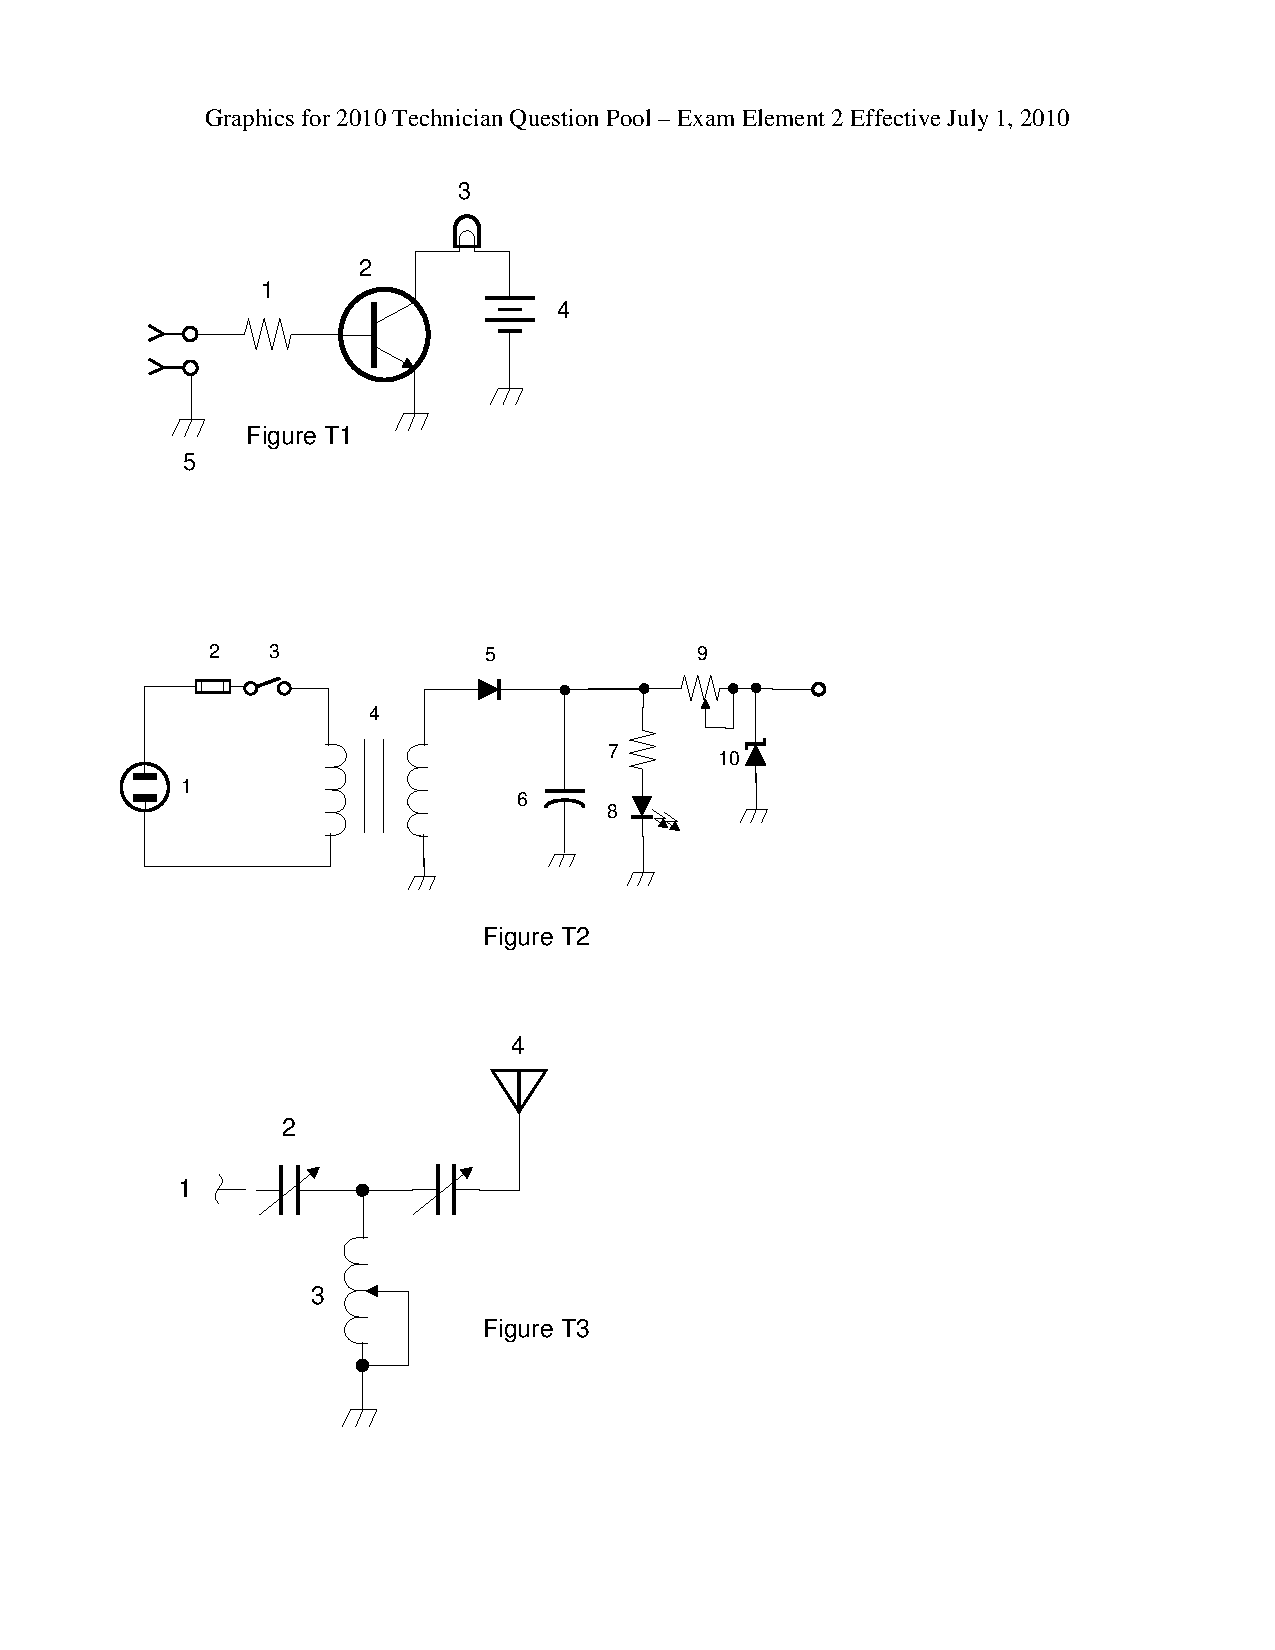
\includegraphics[pages={1},height=.9\textheight]{2010element2graphics.pdf}
\end{frame}

\part{How Radio Works}
\section{Modulations}
\begin{frame}
\frametitle{Modulation}
In radio we use different methods for "encoding" information on electromagnetic waves. All methods take advantage of some of the really cool parts of waves and trig.\\
Yes that math is good for something!
\end{frame}


\subsection{Continuous Wave}
\begin{frame}
\frametitle{CW}
Continuous Wave or CW communicates information by turning a signal on and off. If two parties agree on what different pasterns of On's and Off's mean then they can share information. The most common system is International Morse Code. 
\end{frame}

\begin{frame}
\frametitle{CW picture}
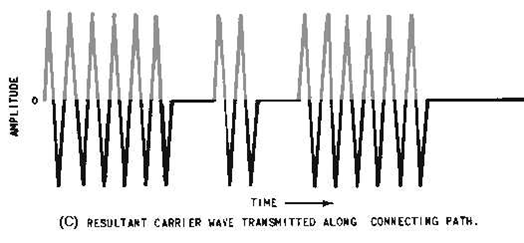
\includegraphics[height=.5\textheight]{cw.png}
\end{frame}

\subsection{Amplitude Modulation}

\begin{frame}
\frametitle{AM}
Amplitude Modulation or AM, works by keeping the frequency of a signal steady and varying the amplitude or intensity of the wave. For sounds, we simply add the sound wave to the radio wave. There are commercial AM stations, generally in lower frequencies bands. AM waves can be subject to many different forms of interference. Next to CW, AM makes for the simplest transmitters and receivers.
\end{frame}

\begin{frame}
\frametitle{AM picture}
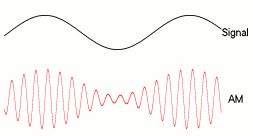
\includegraphics[height=.5\textheight]{am.png}
\end{frame}

\subsection{Single Sideband}

\begin{frame}
\frametitle{SSB }
\begin{columns}
\column{.4\textwidth}
AM is really easy but isn't very efficient. The image to the right shows the power of an AM wave. The center spike is the Carrier, and holds no useful information. The smaller peaks on either side are mirrored across the carrier. If we remove everything but on of the sides we can more efficiently use power and bandwidth. This is called Single Side band
\column{.6\textwidth}
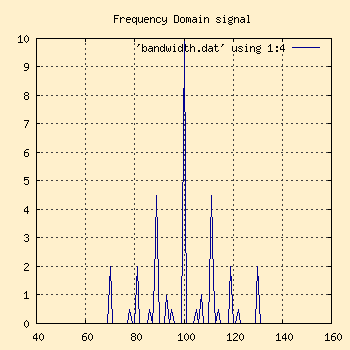
\includegraphics[width=\textwidth]{amfft.png}
\end{columns}
\end{frame}


\begin{frame}
\frametitle{SSB Continued}
From the graph we can see there are two different sidebands, one on either side of the carrier. The one that is higher in frequency is the "Upper" Sideband and the lower one is the "Lower" Sideband. For historical reasons we Upper Sideband (USB) on frequencies higher than 10MHz, and Lower Sideband on frequencies lower than 10MHz. There are also times when we use Vestigial Sideband, that is one and a part sidebands, namely for sending images.
\end{frame}

\subsection{Frequency Modulation}

\begin{frame}
\frametitle{FM}
FM or frequency modulation works by varying the frequency of the signal to encode information. FM takes the most bandwidth in that you have clear enough room on either side of the center frequency to allow for a fully modulated signal.
\end{frame}

\begin{frame}
\frametitle{FM Picture}
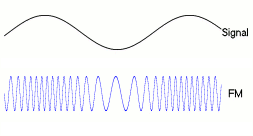
\includegraphics[height=.5\textheight]{fm.png}
\end{frame}

\subsection{Phase Modulation}

\begin{frame}
\frametitle{Phase Modulation}
Related to FM is Phase Modulation. Instead of changing the frequency, we adjust the phase of a signal. The same cirucits that process FM can handle PM.
\end{frame}

\subsection{Extra layers}
\begin{frame}
\frametitle{AFSK, Packett, etc.}
We can add layers on top of these simple modulation systems to encode information. AFSK Audio Frequency Shift Keying, is a digital mode that encodes 0's and 1's as audio tones that can be sent using one of the modulations. Packet radio is a particular protocol for sending information, generally using AFSK. APRS is a way of formatting data send via packet to report the position and other information that can show up on a map.
\end{frame}

\begin{frame}
\frametitle{APRS}
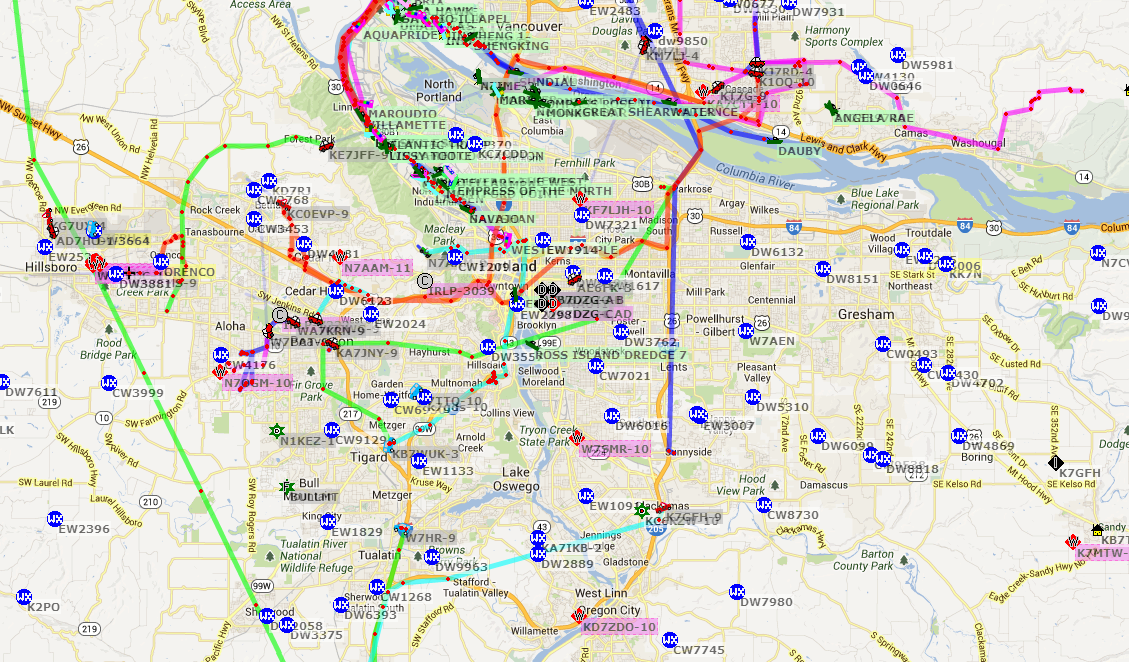
\includegraphics[width=.9\textwidth]{aprspdx.png}
\end{frame}
\section{De-Modulation}

\begin{frame}
\frametitle{De-Modulation}
De-Modulation is the process of extracting information from a radio wave. All receivers are built from the same basic components. The antenna feeds an RF amplifier, A mixer and local-oscillator steps the frequency down to something easier to process, an intermediate frequency (IF). An IF amplifier feeds the de-modulation stage which then into an audio amplifier and out to a speaker. 
\\
It is important to remember that these devices are made of circuits built from the components from the previous section.
\end{frame}

\begin{frame}
\frametitle{Simple Radio}
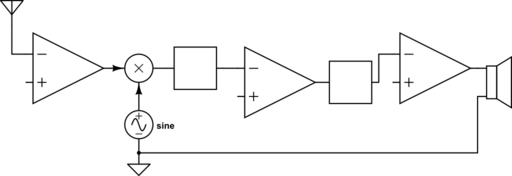
\includegraphics[width=.9\textwidth]{simplereciever.png}
\end{frame}

\subsection{AM}
\begin{frame}
\frametitle{The detector}
The AM demodulation device is called a Detector. Essentially it removes the carrier from the signal and leaves only the information, which for the most part is audio.
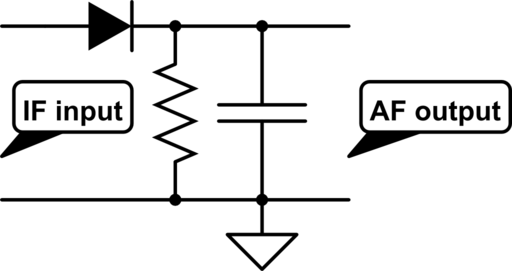
\includegraphics[width=.9\textwidth]{simpledetector.png}
\end{frame}

\subsection{SSB}

\begin{frame}
\frametitle{SSB}
As a SSB signal is just an AM signal without the carrier, it is simple enough to replace it and use the same Detector. An extra component called a Beat Frequency Oscillator is used to replace the carrier that is removed from when transmitting.
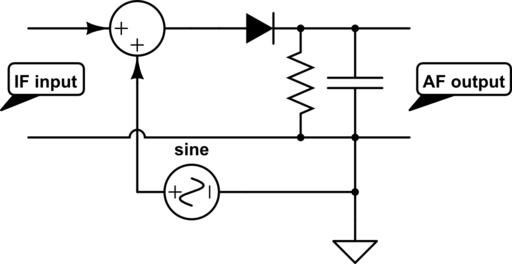
\includegraphics[width=.9\textwidth]{simpleproductdetector.png}
\end{frame}

\subsection{FM}
\begin{frame}
\frametitle{FM}
By far the most complex demodulation circuit is the discriminator used with FM signals. For the purpose of the test you only need to know the type of circuit, not how to build one. 
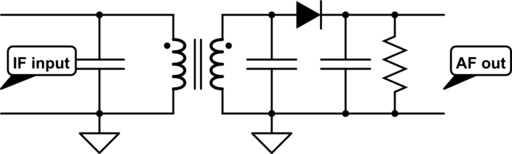
\includegraphics[width=.9\textwidth]{simplediscriminator.png}
\end{frame}

\section{The Transceiver}
\begin{frame}
\frametitle{Modulation and De-modulation together}
For the sake of space it is worth while to combine a transmitter and receiver.
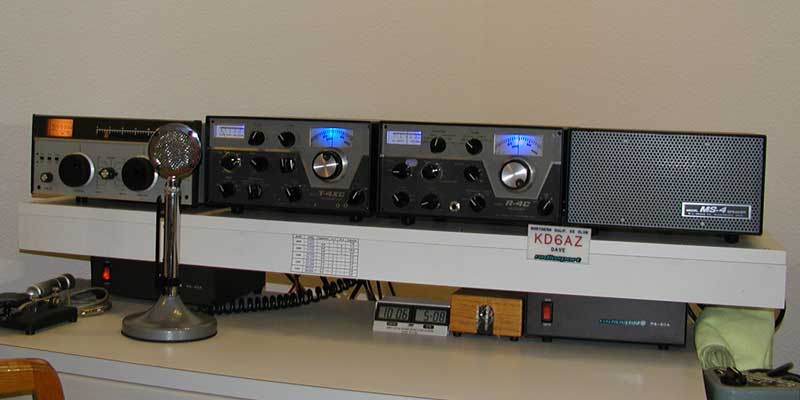
\includegraphics[height=.6\textheight]{drake4.jpg}
\end{frame}

\begin{frame}
\frametitle{Basic}
The simple looking idea is to just hook both a receiver and transmitter to the same antenna, like so.
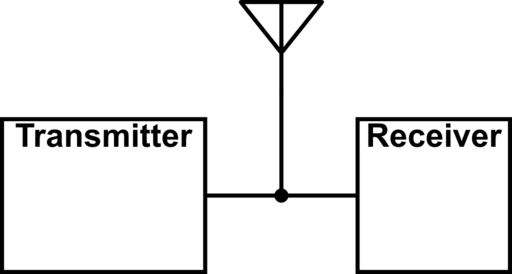
\includegraphics[height=.5\textheight]{simpletr.png}
\end{frame}

\begin{frame}
\frametitle{Real}
The problem with the simple setup is that the energy from the transmitter goes right into the receiver. Remember all those amplifiers in the receiver, they will amplify the very strong signal and then the magic smoke that makes everything work will get out. So \ldots
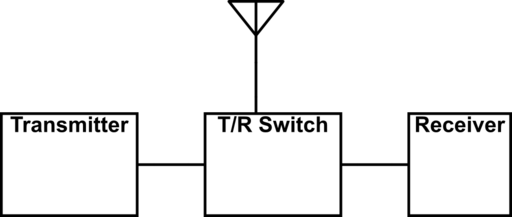
\includegraphics[width=.8\textwidth]{simpletrworks.png}
\end{frame}

\begin{frame}
\frametitle{TR Switch}
The Transmit Receive switch very quickly disconnects either the transmitter or the receiver so that the reliever doesn't blow up.
\end{frame}

\section{Repeaters}

\begin{frame}
\frametitle{Repeaters}
A repeater is just a radio that transmits what it hears. They are generally placed on high places where they can see large areas. They use a technique called Duplex, where it simultaneously receives and transmits on different frequencies. Radios automatically switch between the "input" and "output" frequencies so you don't have to. We often refer to repeaters by their output frequency, and sometimes by their callsign.
\end{frame}

\subsection{Offset}

\begin{frame}
\frametitle{Offset}
The difference between the input, the frequency the repeater listens to, and the output, the frequency the repeater transmits on, is called the offset. The standard offset is part of the band plan. The direction of the offset is also part of the band plan.\\

\begin{tabular}{|l|r|}
\hline
2m & 600 KHz\\ \hline
1.25m & 1.5MHz \\ \hline
70cm & 5MHz \\
\hline
\end{tabular}

\end{frame}

\begin{frame}
\frametitle{Offset Examples}
A couple of sample offsets on 2 meters are.\\
147.16MHz uses a standard positive offset, has an input of 147.76MHz.\\
146.78MHz again with a standard but negative offset has an input of 146.18MHz.\\
It can be difficult to remember if one part of a band is positive or negative so we often write frequency as 147.16+ or 146.78-
\end{frame}

\subsection{Tones}

\begin{frame}
\frametitle{Tones}
Because there is a limited number of locations that are good to place repeaters lots of them end up at the same place. If we don't do anything one can easily cause another to activate. To prevent this we use special signals to make sure we only activate, these are referred to as sub-audible tones.\\

There are two types, CTCSS Continuous Tone Coded Squelch System, and DCS Digital Coded Squelch.
\end{frame}

\begin{frame}
\frametitle{Repeater Directory}
How does one find out information like offset, and tone, and other useful information about a repeater?\\
The ARRL publishes a book called the Repeater Directory.
\end{frame}

\subsection{Duplexing}

\begin{frame}
\frametitle{Duplexers}
Unlike normal radios that don't need to transmit and receive at the same time and can use a switch repeaters inherently have to do both at the same time. The solution is called a duplexer. Duplexers are very selective filters that allow only the transmit frequency between the transmitter and antenna, and only the receive frequency between the antenna and the receiver.
\end{frame}

\begin{frame}
\frametitle{Repeater Picture}
\begin{center}
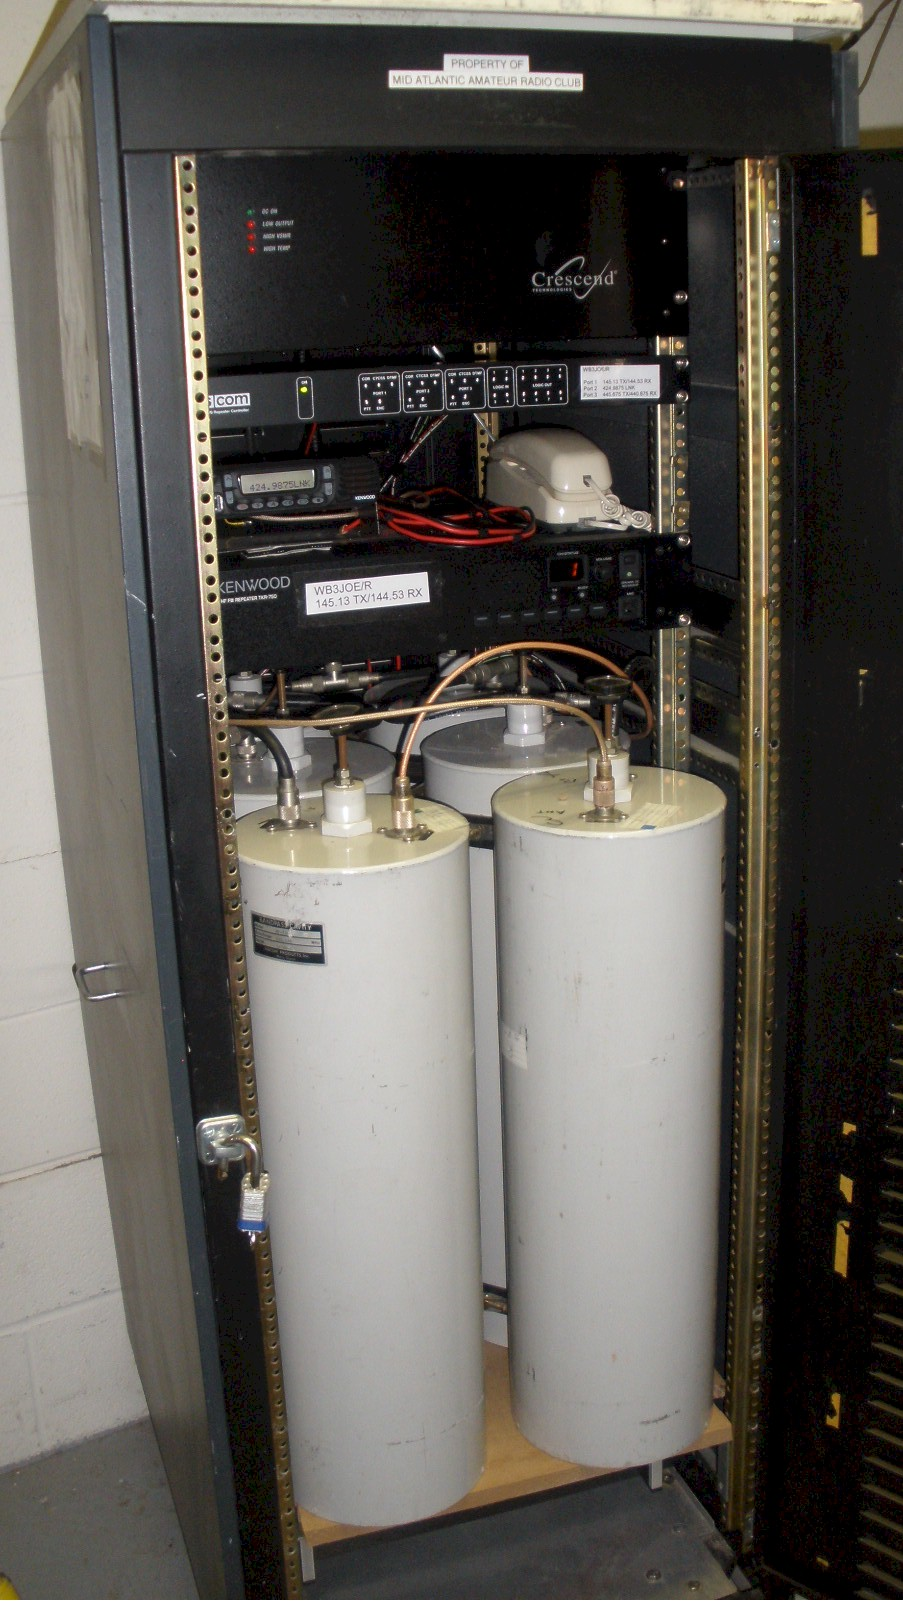
\includegraphics[height=.95\textheight]{repeater.jpg}
\end{center}
\end{frame}

\section{Satellites}

\begin{frame}
\frametitle{Satellite Duplexing}
Remember those large duplexer cans from a repeater that allow transmission and reception on the same band. Well there isn't much extra space on satellites, especially small ones for them. So how do we have satellite repeaters? Simple we separate the transmit and receive frequencies by large margins. The greater the offset the smaller the duplexer can be, when the separation is large enough the device becomes what is known as a diplexer. A diplexer uses simple low-pass and high-pass filters to separate signals from two different bands. More practically they feed different antennas.
\end{frame}

\begin{frame}
\frametitle{Satellite Duplexing}
The convention for describing which bands a satellite operates on uses one or two letters. If there is one letter then the satellite only beacons on that band, if there are two letters the satellite receives on the first letter and transmits on the second. Band letters are H for HF, V for VHF, U for UHF, L for L-band, K for K-band.  Most satellites use mode V/U, meaning they listen on VHF (2-meters) and transmit on UHF (70-cm).
\end{frame}

\subsection{Doppler Shift}
\begin{frame}
\frametitle{Doppler Shift}
Satellites are moving really, really fast, on a few to tens of miles per second. At this speed as they move overhead we have to contend with the Doppler shift, the apparent change in frequency of a wave of emitted by a moving object. As the satellite aproaches the frequency increases, and as it moves away the frequency decreases. This is just like a passing car. The hard part with satellites is the shift you see, is the same shift it sees from you, meaning while you have to tune "up" to hear it when listening, you have to tune "down" so it can hear you.
\end{frame}

\subsection{Tracking}
\begin{frame}
\frametitle{Satellite Tracking}
In order to keep track of where satellites are we use specially formatted numbers called orbital elements. These describe certain aspects of the where a satellite is at. Given these numbers, your location, and the time you can calculate exactly where a satellite is at.
\begin{center}
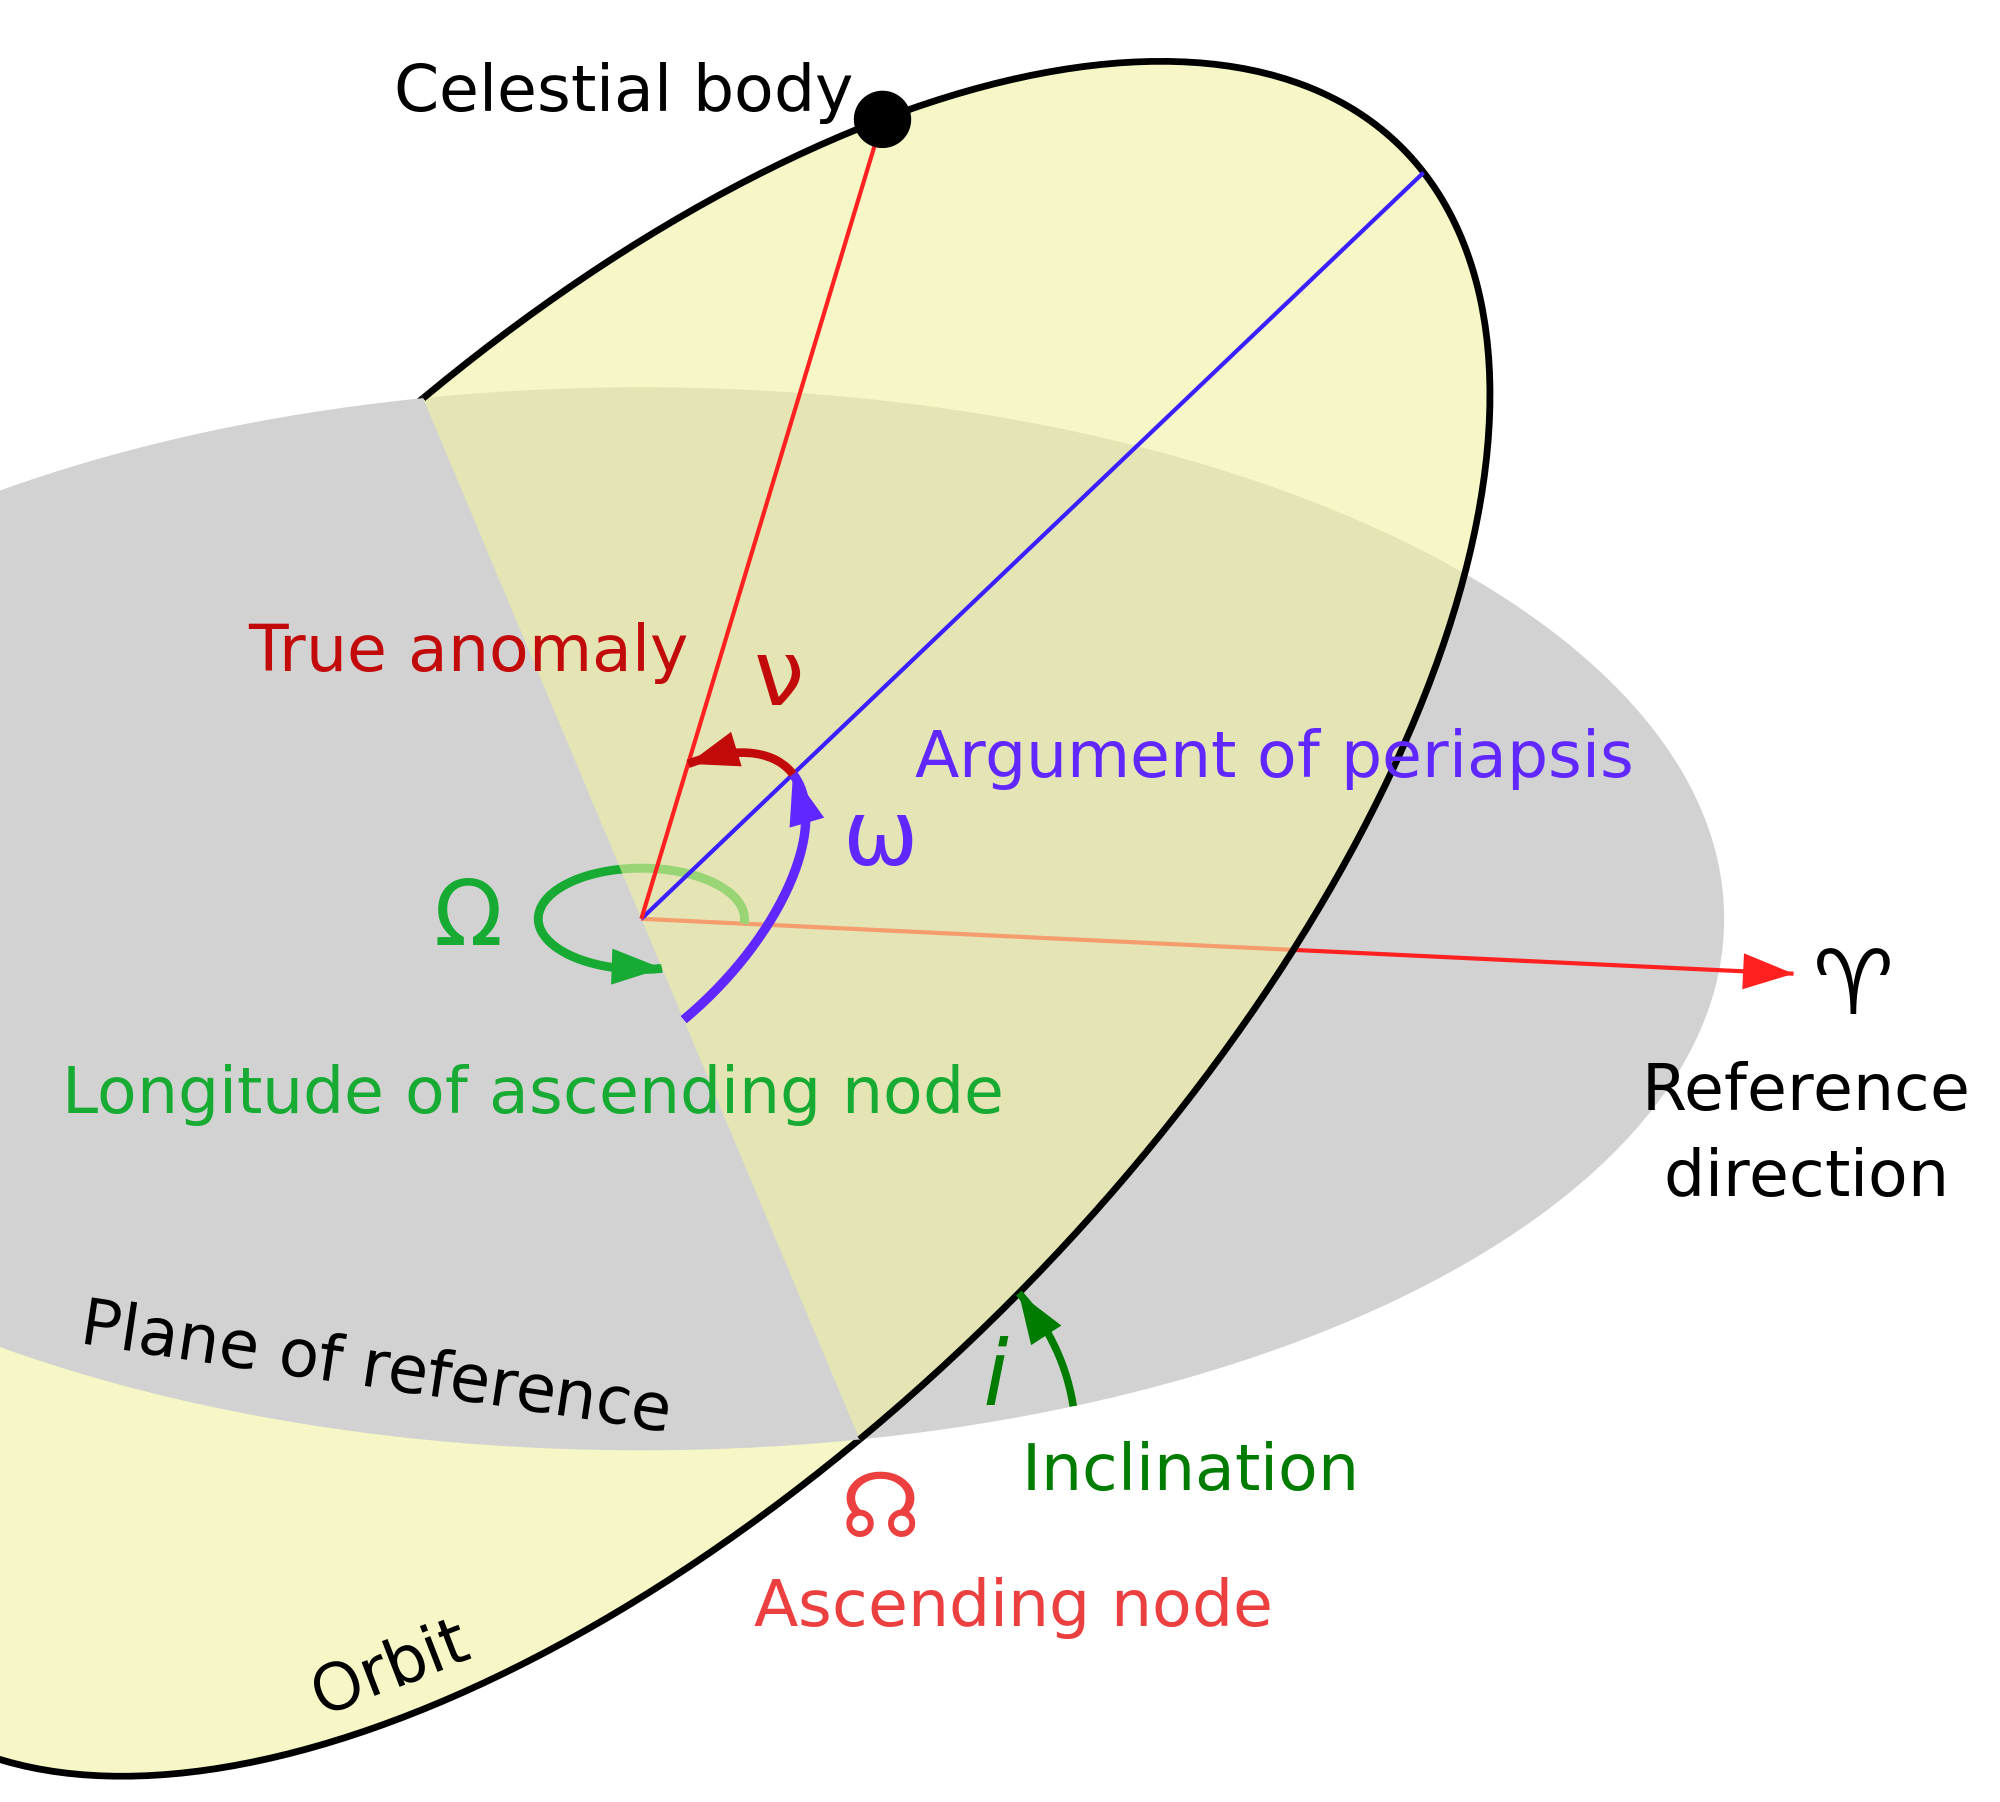
\includegraphics[height=.5\textheight]{orbitelements.png}
\end{center}
\end{frame}

\section{Digital Modes}
\begin{frame}
\frametitle{Its a digital World}
There are many digital modes out there, some encode digital data into digital signals.\\
Some encode analog signals into digital signals.
\end{frame}

\begin{frame}
\frametitle{Baud}
In the digital world there are two important rates.\\
The first is the Baud rate or number of symbols sent per second. In this case a symbol can be a particular tone, or even a change in phase or amplitude.\\
The second is the bit rate, to calculate the bit rate you take the number of bits per symbol and multiply it by the baud rate.\\
Often the bit rate and baud rate are the same, but not always. Some techniques such as Phase Shift Keying can support many bits per symbol.
\end{frame}

\subsection{Digital Voice}
\begin{frame}
\frametitle{Digital Voice}
There are several digital modes that allow analog voice to be sent using digital signals. These are APCO Project 25 (p25), D-STAR, and AOR ARD9800. These all work similarly to cellphones and VoIP.
\end{frame}

\subsection{RTTY}
\begin{frame}
\frametitle{RTTY}
RTTY - Radio TeleTYpe, is the original digital mode. It is slow 50 to 300 baud, or bits per second, that is a single text message in 4-25 seconds. It uses Frequency Shift Keying (FSK) and transmits two tones one for a "high" or 1, and a different one for a "low" or 0. RTTY machines have long been used by military and diplomatic posts, using encryption methods RTTY allows for slow, but reliable communications.
\end{frame}

\subsection{Packet}
\begin{frame}
\frametitle{Packet}
Packet radio uses AFSK generally sent using FM on VHF and above, and SSB on HF. In packet the baud rate is the bit rate. On HF speeds of a whopping 300 baud, and on VHF and up speeds range from the common 1200 baud and the extreme 9600 baud. This translates into 1.2-9.6Kbps, or about 0.5-4.3 MegaBytes per hour, or one seventy-fifth the speed required to stream netflix on the lowest quality setting.
\end{frame}

\begin{frame}
\frametitle{Packet modems}
To use things like packet you need something to MODulate, and to DEModulate signals. Put them together and we get a modem. Many devices add features for controlling things like.\\
\begin{itemize}
\item Mailbox(es)
\item BBS
\item DigiPeaters
\item Addressing
\item Error correction
\end{itemize}
Together we call this a Terminal Node Controller or TNC.
\end{frame}

\begin{frame}
\frametitle{Packet Networks}
Packet networks are configured much like how the internet works, just much smaller. "Users" connect to nodes, these nodes can connect to each other. If there are enough nodes lined up, messages can move over great distances. At times it is possible for messages to move across the country and even the world entirely by bouncing from radio to radio.
\end{frame}

\begin{frame}
\frametitle{The Internet}
There are message handling systems that combine the scale and speed of the internet and the robustness of radio. One such system is Winlink 2000 (yes people still use things like 2000 in names). Nodes in the system decide try to move messages through the internet, and if not over radio, special servers track messages to ensure they get delivered to the appropriate user.
\end{frame}

\subsection{APRS}
\begin{frame}
\frametitle{APRS}
The Automatic Position Reporting System APRS (pronounced A-pers) encodes position data in standard packet formats. Other information such as weather, messages, even icons. The system has "Igates" or internet gateways that pass information to internet servers. \hyperlink{www.findu.com}{findu.com} and \hyperlink{www.aprs.fi}{aprs.fi}
\end{frame}

\section{Linked Repeaters}

\begin{frame}
\frametitle{Linked Repeaters}
Some repeaters are linked using radios, one such system is the Peak Radio Association system. This network allows users all over the state and parts of Washington and California to speak to each other. It does take a second or two for all the links to activate.
\end{frame}

\begin{frame}
\frametitle{IRLP and EchoLink}
The Internet Repeater Linking Project or IRLP connects repeaters using the internet, audio from one repeater are sent to others.\\
Echolink allows users to connect radios, computers, phones, tablets, etc\. to their network. The result is similar to IRLP though you don't have to have a radio to use echolink. 
\end{frame}

\part{Antennas and Feedline}

\section{Antennas}
\begin{frame}
\frametitle{Antennas}
Any radio amateur will tell you that while a million watts is cool, at the end of the day its the antenna that does the real work.\\
Antennas take radio signals in the form of electrons moving in wires and converts that signal into electromagnetic waves, and back.\\
Improperly antenna configurations can even damage your radio! A 5 watt radio with a great antenna can get a lot more work done than 1000 watt radio with a poor antenna.
\end{frame}

\subsection{1/4 Vertical}
\begin{frame}
\frametitle{Quarter Wave Vertical}
\begin{columns}
\begin{column}{.6\textwidth}
Probably the simplest antenna to look at is the 1/4 vertical. It is made of two parts, a vertical section of wire that is 1/4 the wavelength long, and ground.\\
The wavelength is that of the wave in the wire, which is not the same as in free space. Fortunately the math has already been done for us, over and over and the equation is: $L\left(ft\right) = \frac{234}{F \left(MHz\right)}$
\end{column}
\begin{column}{.4\textwidth}
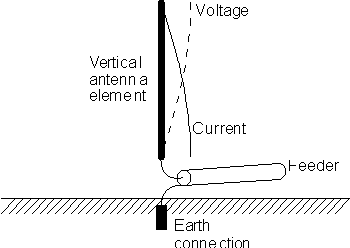
\includegraphics[width=\textwidth]{qwavevert.png}
\end{column}
\end{columns}
\end{frame}

\begin{frame}
\frametitle{Grounding}
\begin{columns}
\begin{column}{.5\textwidth}
The problem with this is that the antenna needs to be close to ground, but we want antennas to be really high up so they can "see" further.\\
The solution is to create a "fake" ground that can elevated with the vertical section.
\end{column}
\begin{column}{.5\textwidth}
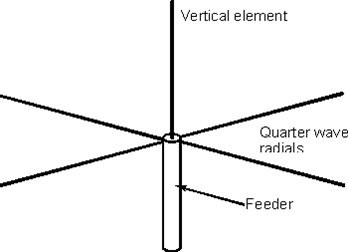
\includegraphics[width=\textwidth]{qwavevertwground.png}
\end{column}
\end{columns}
\end{frame}

\begin{frame}
\frametitle{Vertical Radiation Patern}
The vertical radiates well in all horizontal directions, but doesn't do very well up or down.
\begin{center}
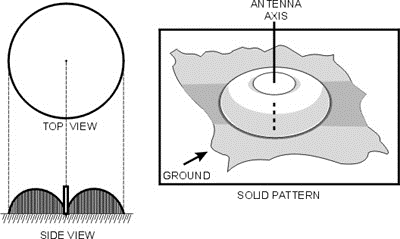
\includegraphics[height=.7\textheight]{qwavevertrad.png}
\end{center}
\end{frame}

\subsection{1/2 Wave Dipole}

\begin{frame}
\frametitle{1/2 Wave Dipole}
Another common antenna is the 1/2 wave dipole. This is made by placing two 1/4 wave wires in lines and feeding them in the middle. This uses one of the wires as the "ground". The total length is twice that found for the 1/4 vertical.
\begin{center}
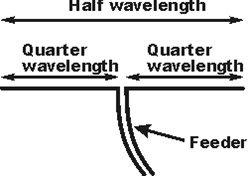
\includegraphics[height=.5\textheight]{hwavedipole.png}
\end{center}
\end{frame}

\begin{frame}
\frametitle{Dipole Radiation patern}
The dipole radiates well perpendicular to the length of the wire. A dipole running north-south will radiate east-west.
\begin{center}
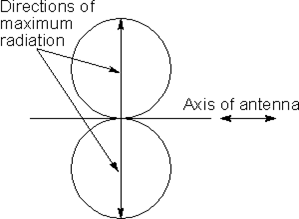
\includegraphics[height=.5\textheight]{hwavedipolerad.png}
\end{center}
\end{frame}

\subsection{Gain}
\begin{frame}
\frametitle{Gain}
\begin{columns}
\begin{column}{.5\textwidth}
The yellow dot and line are the antennas. The red circle is the radiation pattern of the vertical, and the green circles are the pattern for the dipole. The distance from the center indicates the strength.\\
Notice how the dipole is better in two directions but worse the other two. The apparent increase in signal strength when the dipole is "pointed" in the right direction is called Gain.
\end{column}
\begin{column}{.5\textwidth}
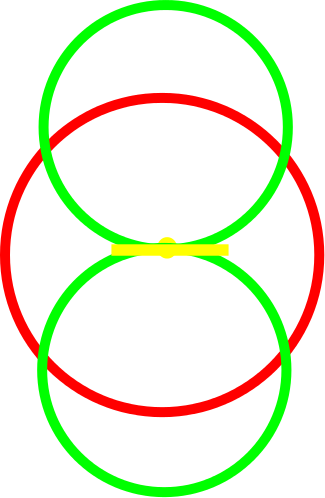
\includegraphics[width=\textwidth]{vertvsdipole.png}
\end{column}
\end{columns}
\end{frame}

\begin{frame}
\frametitle{dB's}
We generally measure Gain in terms of decibels, dB. This is a ratio measurement, meaning it compares two things. We often will compare antennas to an "isotropic" antenna or a perfect 1/2 wave dipole, dBi and dBd. If an antenna claims some gain without saying what it is compared to ASK!. for POWER the equation is $dB=10\log\frac{P}{P_0}$ and for voltage its $dB=20\log\frac{V}{V_0}$ where P and V are your apparent signal and $P_0$ and $V_0$ are the starting points.\\
A good rule to remember is that a change of 3dB in power is a change of a factor of 2 for power, and a change of 6dB is a factor of 2 for voltage. We almost always talk in terms of power.
\end{frame}

\subsection{The Yagi}
\begin{frame}
\frametitle{The Yagi-Uda}
If we add another length of wire behind the dipole to reflect incoming signals into the antenna, and more in front to direct signals we get a Yagi-Uda, or Yagi.\\
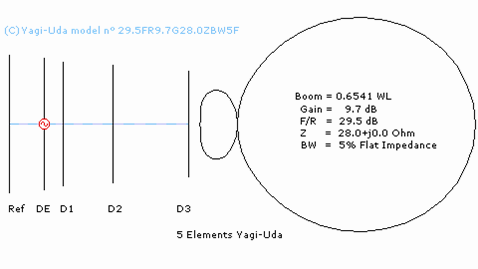
\includegraphics[height=.5\textheight]{yagi.png}
\end{frame}

\begin{frame}
\frametitle{Giant Antennas}
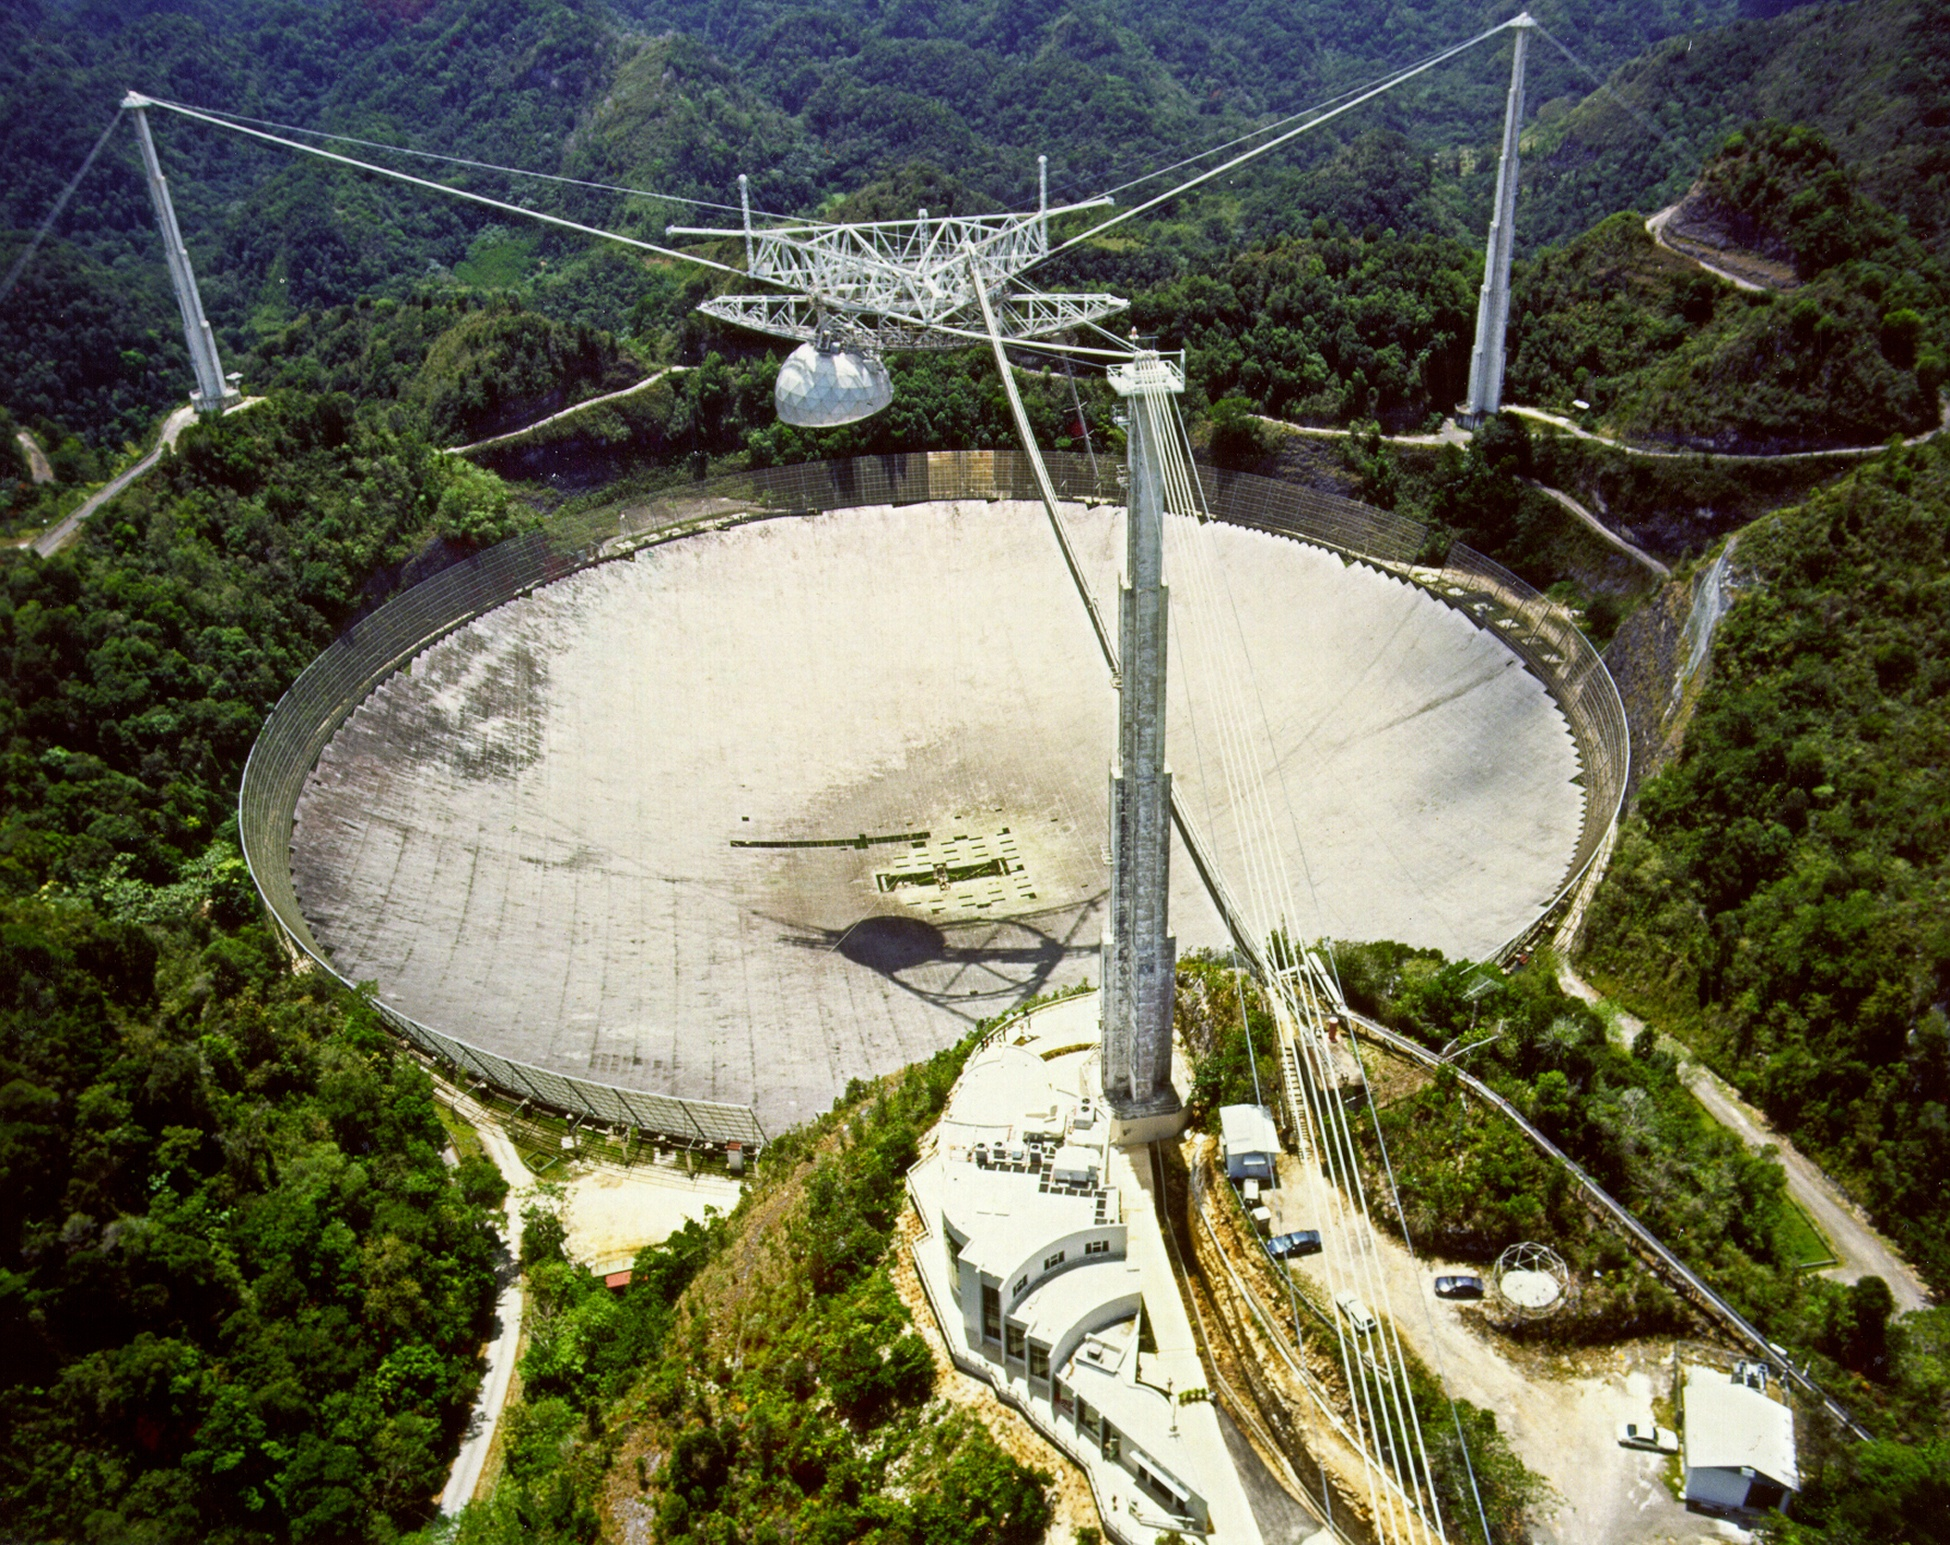
\includegraphics[width=.49\textwidth]{arecibo.jpg}
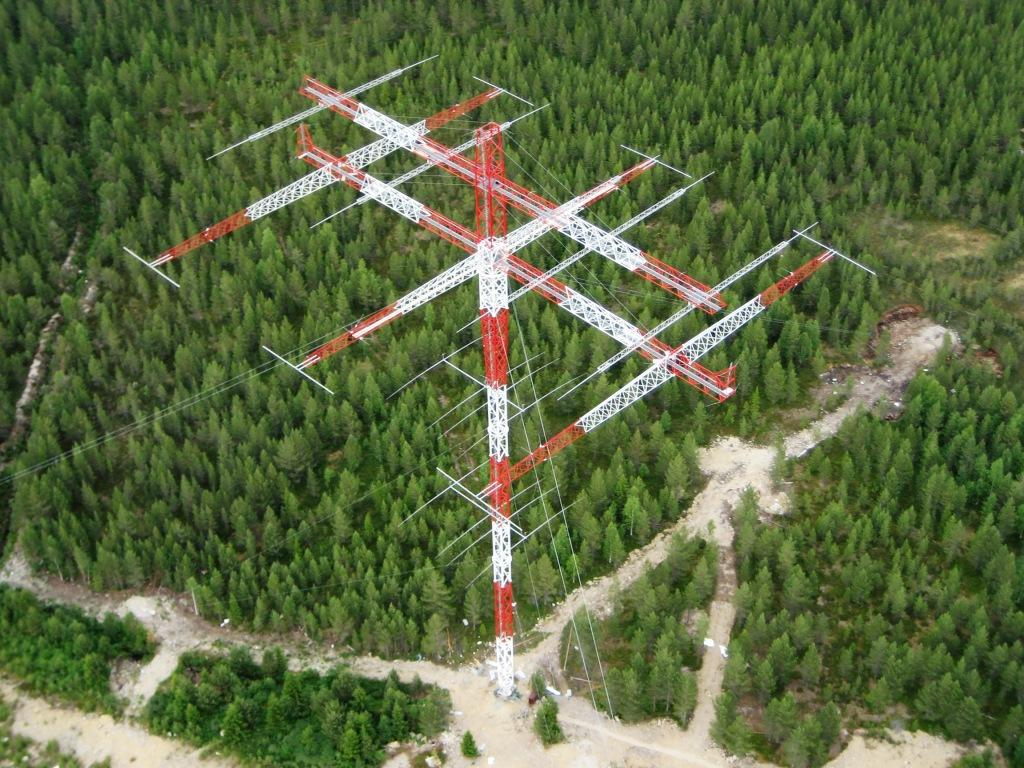
\includegraphics[width=.49\textwidth]{160myagi.jpg}
\end{frame}

\section{Feedline}
\begin{frame}
\frametitle{Feed Me!}
Antennas need a connection to the radio. We call this connection "feedline". It has one job, carry the signal between the radio and antenna as efficiently as possible.
\end{frame}

\subsection{Waveguide}
\begin{frame}
\frametitle{Wave Guide}
One type of feedline is the waveguide, which is really just a hollow tube in which a signal bounces off the walls as it moves from end to end. Fiber optic cables are an example of a waveguide for light. In the waveguide the signal moves as a radio wave. The size of the guide depends on the wavelength of the wave, they are almost never used below UHF as they get really really big. 
\end{frame}

\subsection{Coaxial Cable}
\begin{frame}
\frametitle{Coax}
By far the most common feedline in use is Coaxial Cable. They are made of a center wire surrounded by an insulator, which is in turn surrounded by a metal shield and another outer insulator. More layers of shields and insulators can be added as needed. The term Coaxial refers to the fact that all the components share a common axis.
\end{frame}

\begin{frame}
\frametitle{More Coax}
Coax has several advantages over other feedlines. It is generally flexible and the metal shield and outer insulator allows it to go almost anywhere, even underground. However it is important to watch out for kinks, damage to the insulation and water.\\
Once water gets into the cable it is done for, it corrodes the metal components, and changes the properties of the cable.
\end{frame}

\begin{frame}
\frametitle{Hardline}
One type of coax is called hardline, it is not flexible. It is very low loss, can be pressurized to keep water out, and is less affected by water in the first place.\\
However it is hard to work with, it requires special equipment, its is heavy and very expensive.\\
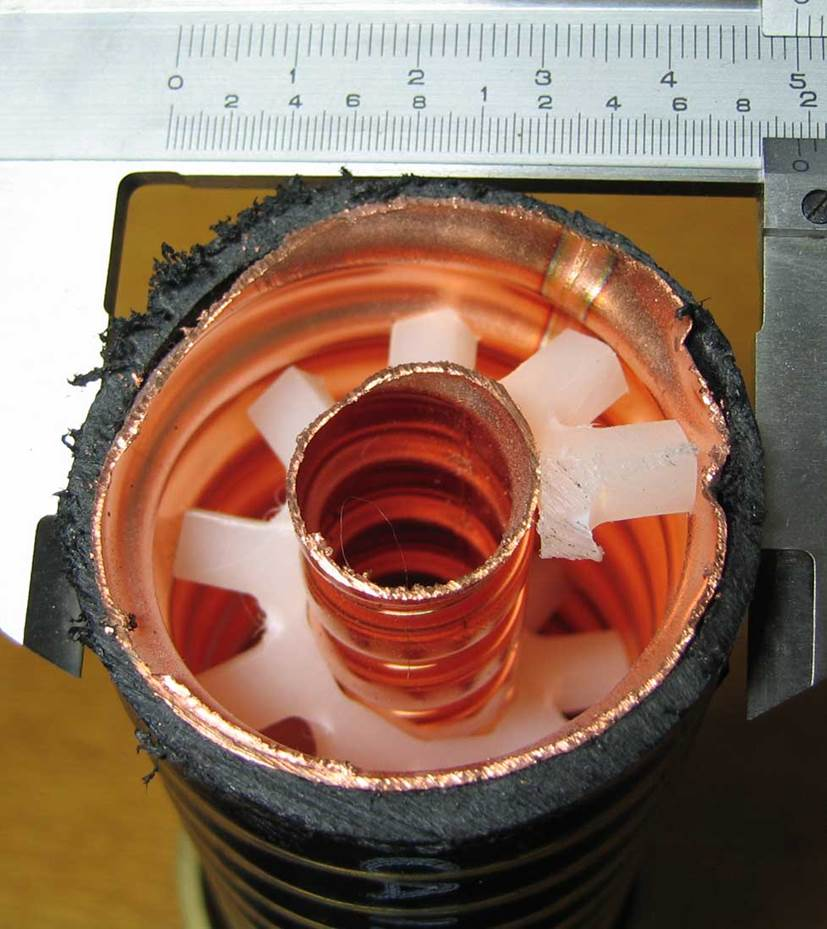
\includegraphics[height=.4\textheight]{4inhardline.jpg}
\end{frame}

\begin{frame}
\frametitle{Losses}
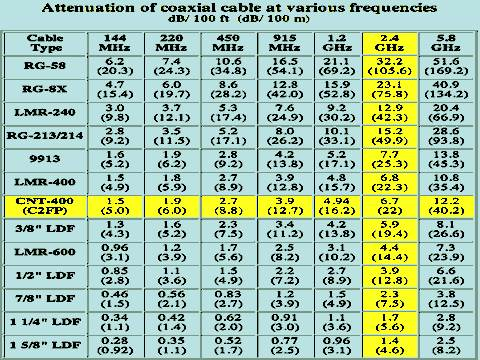
\includegraphics[height=.9\textheight]{coaxatten.jpg}
\end{frame}

\section{Impedance}
\begin{frame}
\frametitle{Impedance}
Impedance is the opposition to the flow of current in an AC circuit (e\.g\. RF). It is a combined measure of the ohmic resistance, capacitance, and inductance of a circuit. Antennas have an impedance, feedlines are designed to have a known impedance, and radios have input and output impedance.\\
Common impedance measurements in amateur radio are 50$\Omega$ and 300$\Omega$, while TV cables are normally 75$\Omega$ 
\end{frame}

\begin{frame}
\frametitle{Impedance Matching}
If there is a mismatch in impedance then power will reflect from the point of the mismatch. This is bad! signals from the antenna bounce back to the antenna and don't reach the radio. Even more dire strong signals from the radio don't make it to the antenna and bounce back into the radio!\\
The most efficient systems match impedance as closely as possible.
\end{frame}

\begin{frame}
\frametitle{The SWR meter}
A simple tool for checking impedance matches is the SWR meter, they simply show you the ratio of power going out to power coming back. A match of 1:1 is perfect, most things will work with a mismatch of up to 2:1, any higher and there is a real problem.
\end{frame}

\begin{frame}
\frametitle{Check everything first}
So a good SWR means all is good right? \pause Well not exactly\ldots \\\pause
Lets say you have a 50W radio and a broken antenna with really lossy cable say 10.6dB.\\
When it reaches the antenna and reflects back it is down to 4.3W and radio only sees 0.4W.\\
$SWR=\frac{F+R}{F-R}=\frac{50.4}{49.6}=1.01:1$\\
This is a great SWR but all the power is going into the cable. The radio will be happy but you have just made your feedline a 50W heater.
\end{frame}

\begin{frame}
\frametitle{Title}

\end{frame}

\begin{frame}
\frametitle{Title}

\end{frame}

\begin{frame}
\frametitle{Title}

\end{frame}

\begin{frame}
\frametitle{Title}

\end{frame}

\begin{frame}
\frametitle{Title}

\end{frame}

\begin{frame}
\frametitle{Title}

\end{frame}

\begin{frame}
\frametitle{Title}

\end{frame}

\begin{frame}
\frametitle{Title}

\end{frame}

\begin{frame}
\frametitle{Title}

\end{frame}

\begin{frame}
\frametitle{Title}

\end{frame}

\begin{frame}
\frametitle{Title}

\end{frame}

\begin{frame}
\frametitle{Title}

\end{frame}

\begin{frame}
\frametitle{Title}

\end{frame}

\begin{frame}
\frametitle{Title}

\end{frame}

\begin{frame}
\frametitle{Title}

\end{frame}

\begin{frame}
\frametitle{Title}

\end{frame}

\begin{frame}
\frametitle{Title}

\end{frame}

\begin{frame}
\frametitle{Title}

\end{frame}

\begin{frame}
\frametitle{Title}

\end{frame}

\begin{frame}
\frametitle{Title}

\end{frame}

\begin{frame}
\frametitle{Title}

\end{frame}

\begin{frame}
\frametitle{Title}

\end{frame}

\begin{frame}
\frametitle{Title}

\end{frame}

\begin{frame}
\frametitle{Title}

\end{frame}

\begin{frame}
\frametitle{Title}

\end{frame}

\begin{frame}
\frametitle{Title}

\end{frame}

\begin{frame}
\frametitle{Title}

\end{frame}

\begin{frame}
\frametitle{Title}

\end{frame}

\begin{frame}
\frametitle{Title}

\end{frame}

\begin{frame}
\frametitle{Title}

\end{frame}

\begin{frame}
\frametitle{Title}

\end{frame}

\begin{frame}
\frametitle{Title}

\end{frame}

\begin{frame}
\frametitle{Title}

\end{frame}

\begin{frame}
\frametitle{Title}

\end{frame}
%
%\begin{frame}
%\frametitle{Title}
%hello world
%\end{frame}
%
\end{document}